\documentclass[oneside,bibliography=totocnumbered,BCOR=5mm]{scrbook}

\usepackage[ngerman]{babel}
\usepackage{fontspec}

% look up system fonts via fc-list
% \setmainfont
\setsansfont{SFNS Display}
\setmonofont{FuraCode Nerd Font Mono}
% see: jneidel.com/dot/.fonts

\usepackage[
backend=biber,
bibstyle=authoryear,
citestyle=authoryear,
autocite=footnote
]{biblatex}
\addbibresource{bibliography.bib}
\addbibresource{extra.bib}

\usepackage{graphicx}
\graphicspath{ {images/} }
\usepackage{float} % [H] on images to have them 'here'

\usepackage[newfloat]{minted}
\usepackage[hang, small,labelfont=bf,up,textfont=it,up]{caption}

\newenvironment{code}{\captionsetup{type=listing, skip=0pt}}{}
\SetupFloatingEnvironment{listing}{name=Listing}

\newminted{shell}{
  linenos,
  numbersep=6pt,
  frame=lines,
  framesep=2mm,
  fontsize=\footnotesize
}
\newminted{javascript}{
  linenos,
  numbersep=6pt,
  frame=lines,
  framesep=2mm,
  fontsize=\footnotesize
}
\newmintinline[codeinline]{shell}{
  fontsize=\small
}
\newmintinline[codeinlinefn]{shell}{ % footnote
  fontsize=\scriptsize
}

\usepackage{marvosym}
\usepackage{csquotes}
\usepackage{hyperref}
\usepackage{microtype} % Slightly tweak font spacing for aesthetics
\usepackage{nameref}

\usepackage[hmarginratio=1:1,top=32mm,columnsep=20pt]{geometry} % Document margins
\usepackage{booktabs} % Horizontal rules in tables
\usepackage{lettrine} % The lettrine is the first enlarged letter at the beginning of the text
\usepackage{enumitem} % Customized lists
\setlist[itemize]{noitemsep} % Make itemize lists more compact

\usepackage{fancyhdr} % Headers and footers
% \pagestyle{fancy} % All pages have headers and footers
\fancyhead{} % Blank out the default header
\fancyfoot{} % Blank out the default footer

\usepackage{titling} % Customizing the title section

\begin{document}

% Titelseite
% \pagestyle{empty} % keine Seitennummer
\begin{titlepage}
\begin{center}

\includegraphics{htw-logo.jpg}
\linebreak[4]
\linebreak[4]
\linebreak[4]
\linebreak[4]
\textit{\large Entwicklung und Evaluation von Methoden zur Absenkung der Nutzungsschwelle von Kommandozeilen-Interfaces}
\linebreak[4]
\linebreak[4]
\linebreak[4]
Abschlussarbeit
\linebreak[4]
\linebreak[4]
zur Erlangung des akademischen Grades:
\linebreak[4]
\linebreak[4]
\textbf{Bachelor of Science (B.Sc.)}
\linebreak[4]
\linebreak[4]
an der
\linebreak[4]
\linebreak[4]
Hochschule f\"ur Technik und Wirtschaft (HTW) Berlin
\linebreak[4]
Fachbereich 4: Informatik, Kommunikation und Wirtschaft
\linebreak[4]
Studiengang \textit{Angewandte Informatik}
\linebreak[4]
\linebreak[4]
\linebreak[4]
1. Gutachter: Prof. Dr.-Ing. Johann Habakuk Israel\linebreak[4]
2. Gutachter: B.Sc. Moritz Wachter\linebreak[4]
\linebreak[4]
\linebreak[4]
\linebreak[4]
\linebreak[4]
Eingereicht von Jonathan Neidel \textit{(573619)}
\linebreak[4]
\linebreak[4]
\linebreak[4]
\linebreak[4]
13. Februar 2023

\end{center}
\end{titlepage}
\newpage

\thispagestyle{empty}
\vspace*{2.2cm}
\noindent
{\Huge Danksagung}\\
\vspace*{1.6cm} \\

%\pagestyle{headings} % Kopfzeilen (automatisch erzeugt)

An Endava für die Möglichkeit die Arbeit im Betrieb zu schreiben.

\medskip

An Moritz der dies ermöglicht hat und mir helfend zur Seite stand.

\medskip

An Herr Israel für die Beantwortung aller aufkommenden Fragen.

\medskip

An Francis und meine Mutter für den moralischen Support.

\newpage
\thispagestyle{empty}

\section*{Abstract}

Diese Arbeit beschäftigt sich mit der Verbesserung von Anwendungen mit
Kommandozeilen-Inferfaces, kurz CLI Apps. Zur Optimierung deren Usability wurden
die zwei zugrunde liegenden Probleme aufgezeigt. Es wurden anwendbare Methoden
erarbeitet, welche diese Probleme mitigieren sollen.

Die Umsetzung dieser Methoden wurde an einer Beispielanwendung durchgeführt, um
Details und Komplikationen in der Implementierung aufzuzeigen. Darüber hinaus
wurden Performance und Attraktivität verglichen, indem die Kommandozeilen
Anwendung einer grafischen gegenüber gestellt wurde.

Im Vergleich bevorzugten die sechs Teilnehmer die vergleichbare Performance als
auch die bessere Nutzbarkeit des Kommandozeilen-Interfaces.

\clearpage
\pagenumbering{roman}
\tableofcontents
.
\newpage

\pagenumbering{arabic}
\chapter{Einleitung}
\label{sec:einleitung}

\section{Hintergrund der Arbeit}

Diese Arbeit setzt sich mit dem Kommandozeilen-Interface auseinander. Laut
\cite{Raskin_2008} ist es ``still one of the most powerful interface paradigms
we have for controlling our computers.''. Gleichzeitig ist es aber auch als
traditionelles Interface Teil der Computergeschichte \parencite{nielson1993}.
Damit einher gehen Probleme und Schwächen.

\section{Problem- und Zielstellung}
% [Beschreibung der Problemstellung sowie der sich daraus ergebenden Teilprobleme,-ziele und Forschungsfrage(n), welche Sie mit Ihrer Arbeit addressieren]

\label{sec:problem}

Das Kommandozeilen-Interface ist heutzutage ein wenig verbreitetes
Anwendungs-Interface. Besonders in der allgemeinen Bevölkerung, aber selbst
unter Entwicklern werden für die meisten Anwendungsfälle grafische Apps
bevorzugt.

Das sich daraus ergebende Problem ist: Wie kann das Kommandozeilen-Interface
Entwicklern oder der Allgemeinheit näher gebracht werden? Das Teilproblem
im Fokus dieser Arbeit sind die Probleme in der Nutzbarkeit die ein
Kommandozeilen-Interface mit sich bringen kann.

Ziel ist es implementierbare Methoden zum Verbessern der Usability von
Anwendungen mit Kommandozeilen-Interface zu entwickeln. Die Anwendung dieser
sollte die Nutzungsschwelle von Kommandozeilen Apps abzusenken und an die
Usability von alternativen, meist grafischen Anwendungen angleichen. Um dies
zu demonstrieren sollen die entwickelten Methoden in einem Anwendungsbeispiel
implementiert und in einer Evaluation mit einer grafischen Alternative
verglichen werden.

\newpage
\section{Aufbau der Arbeit}

\begin{enumerate}
  \item \textbf{\nameref{sec:einleitung}}
    \smallbreak
    Definieren der Ziele und Struktur.
  \item \textbf{\nameref{sec:grundlagen}}
    \smallbreak
    Beschreiben grundlegenden Wissens.
  \item \textbf{\nameref{sec:cli-problems}}
    \smallbreak
    Zusammenfassen von Problemen, welche das Nutzen von Kommandozeilen-Interfaces erschweren.
  \item \textbf{\nameref{sec:methods}}
    \smallbreak
    Formulieren von Methoden um die zuvor geschilderten Probleme adressieren.
  \item \textbf{\nameref{sec:beispiel-anwendung}}
    \smallbreak
    Definieren und Bauen einer CLI App als Beispiel zur Anwendung der Methoden.
  \item \textbf{\nameref{sec:implementation}}
    \smallbreak
    Beschreiben von Details und Schwierigkeiten bei der Implementierung der Methoden.
  \item \textbf{\nameref{sec:evaluation}}
    \smallbreak
    Durchführen einer vergleichenden Studie zwischen der implementierten CLI App
und einer funktionell gleichen\footnote{Im Kontext der Studie wird nur die von
beiden Anwendungen überlappende Funktionalität getestet und verglichen.} GUI
Webapp.
  \item \textbf{\nameref{sec:zusammenfassung}}
    \smallbreak
    Ziehen einer Schlußfolgerung.
\end{enumerate}

\chapter{Grundlagen}
\label{sec:grundlagen}

\section{Historischer Kontext}
\label{sec:historic-context}

Die Kommandozeile ist ein Produkt der Evolution von Computern. Die ersten
Formen der Interaktion in Echtzeit kamen zusammen mit dem `teletypewriter'
(TTY), einem Schreibmaschinen-ähnlichem Gerät. Erstmals konnten Menschen
ihre Befehle eingeben und die direkt die Resultate sehen. Das Papier und die
mechanischen TTY's wurden schließlich durch text-darstellende Displays und
elektronische Tastaturen ersetzt. Diese Interaktionsform mit Tastatur und
Textausgabe ist als \textbf{Kommandozeilen-Interface (CLI)} bekannt geworden
\parencite[35f]{nagarajan2018}. Und funktioniert wie folgt:

\begin{enumerate}
  \item Das System fordert den Nutzer auf einen Programmaufruf zu schreiben. (`Read')
  \item Das System führt den Befehl aus und zeigt das Resultat. (`Eval' und `Print')
  \item Diese Sequenz wiederholt sich nun unendlich. (`Loop')
\end{enumerate}

Ein System das dieses Vorgehen implementiert, wird auch als REPL
(`Read-eval-print loop`) Umgebung bezeichnet.

Um die Limitation der Kommandozeile\footnote{Im Kapitel \ref{sec:cli-problems}
wird noch tiefer auf die Probleme eingegangen.} zu adressieren, wurde
unter anderem das grafische User Interface (\textbf{GUI}) entwickelt
\parencite{nielson1993}. Welches von dem text-basierten CLI zu dem
heute allgegenwärtigen Fenster, `Icons', Menüs und die Maus mit sich
brachte\footnote{Mehr zu den Weiterentwicklung des CLI in Kapitel
\ref{sec:weiterentwicklungen}.}

\section{Vorteile der Kommandozeile}

Das CLI bietet Experten viel Flexibilität konstruieren eines (komplexen)
Operation \parencite{Norman_1983}. Ein Beispiel für diese Flexibilität wäre
folgendes. Es sollen alle PDF Dateien aus dem Jahr 2021 gelöscht werden, diese
haben etwa Namen wie: \codeinline{20210819-Rechnung.pdf}. In der Kommandozeile
kann dies mit \codeinline{rm 2021*.pdf} erreicht werden. Im grafischen Interface
müssten die Dateien markiert und gelöscht werden. Mit einer steigender Anzahl
von Dateien steigt auch der Aufwand und die Chance einen Fehler zu machen.
In der Shell funktioniert \codeinline{rm} auch problemlos bei einer Million
Dateien.

Ein weiter Vorteil für Experten liegt in dem Erstellen von Skripten. Mit Hilfe
dieser können Operationen automatisiert werden. Wenn z.B. eine der Rechnungen
aus dem letzten Paragraphen heruntergeladen wurde, kann diese mittels Skript
umbenannt, in den richtigen Ordner verschoben und der Todoliste ein Eintrag à la
`Rechnung xy begleichen' hinzugefügt werden. In einer graphischen Umgebung ist
diese Art von präziser Automatisierung nicht so einfach möglich.

Experten mit viel Wissen und Erfahrung mit dem System wissen meist exakt
welche Operation angewandt werden muss. In der Kommandozeile kann dies einfach
und direkt eingetippt werden. Während selbst Experten in grafischen und
Menü-basierten Interfaces sich immer durch die gleichen Menüs und Untermenüs
klicken müssen.

Als Text-basiertes Interface kommt der Kommandozeile die Klarheit von Worten
zugute. Abstrakte Konzepte wie Marxismus lassen sich nur schwer bis gar nicht in
Bildern beschreiben \parencite{Raskin_2008}, sind aber als Wort sehr umgänglich.

\section{Die Terminal Umgebung}

Die moderne Kommandozeile existiert nicht mehr in Isolation. Um auf diese in
einem grafischen Fenstersystem zugreifen zu können, wird ein \textbf{Terminal
Emulator} benötigt. Wie der Name schon preisgibt: es soll ein traditionelles
text-basiertes Terminal nachgebildet werden. Als grafische Anwendung besteht
aber der Vorteil die Maus zum Klicken oder Markieren verwenden zu können. In
diesem Terminal läuft eine Shell. So nennt man das Programm, welches die Befehle
entgegennimmt und deren Resultate ermittelt und ausgibt. Am weitesten verbreitet
sind Unix Shells wie \codeinline{bash} oder \codeinline{zsh}.
% TODO: Unix?
Die Sprache der Shell gesprochen ist `Shell Script'. Dessen Funktionsumfang
variiert je nach Shell-Dialekt. Die meisten Unix Shells implementieren aber den
POSIX Standard und teilen deshalb eine gewisse Grundfunktionalität. DOS und
andere Windows Shells sind hier außen vor. Diese teilen weder Funktionalität
noch Core Utilities mit den Unix Shells. Die \codeinline{coreutils} sind
Grundlegende Werkzeuge zur Datei- und Textmanipulation \parencite{coreutils},
wie z.B. \codeinline{ls}, \codeinline{cat} oder \codeinline{rm}.

% TODO: more citations
% TODO: unix philsophy here

Neben der Shell gibt es noch andere Kommandozeilen Umgebungen. So gibt es
für viele Programmiersprachen eine Kommandozeile (z.B. für Node.js, Python
oder Scala). In diesen können dann nach gleichem REPL Schema Befehle in der
Programmiersprache interaktiv geschrieben und ausgeführt werden.

\section{Begrifflichkeiten der Kommandozeile}

Für ein Verständnis des CLI sind ein paar Begriffe zu definieren. Ein Shell
Befehl kann auf seine Einzelteile herunter gebrochen werden:

\begin{code}
  \begin{shellcode}
$ cd Downloads
$ git commit -m "Inital commit"
  \end{shellcode}
\end{code}

Das \codeinline{\$} zu Beginn bezeichnet, dass nachfolgend Shell Code kommt. In
der ersten Zeile ist \codeinline{cd} das Kommando, was verwendet werden soll,
gefolgt von einem Argument, etwas das dem Kommando übergeben wird, in diesem
Falle der Name eines Ordners (names \codeinline{Downloads}.) Die Reihenfolge
ist dabei bei mehreren Argumenten entscheidend. In der zweiten Zeile wird
dem \codeinline{git} Kommando das Subkommando \codeinline{commit} übergeben
(\textcite{nagarajan2018}, \textcite{clig}.)

Nicht alle Kommandozeilen Apps haben Subkommandos. \textcite{12factor} definiert
zwei verschiedene Arten von CLI Anwendungen: ``single and multi-command''. Also
klassische `UNIX-Style' Werkzeuge wie \codeinline{cd}, \codeinline{cp} oder
\codeinline{grep}. Und jene Apps mit Subkommandos wie \codeinline{npm} oder
\codeinline{git}, die meist moderner und komplexer sind.

Zurück zu obigen \codeinline{git} Befehl: Dem \codeinline{commit} Subkommando
wird die \codeinline{-m} Flagge und mit ihr ein Parameter (die Nachricht
\codeinline{Inital commit}) übergeben. Die \codeinline{-m} Flagge ist die
Kurzversion der langen \codeinline{--message} Flagge. Kurze Flaggen bestehen
immer aus Bindestrich und einem Buchstaben. Lange Flaggen starten mit zwei
Bindestrichen gefolgt von einem oder mehr Wörtern (meist sind mehrere Wörter
auch durch Bindestriche verbunden, z.B. \codeinline{--non-interactive}.)
Funktionell sind beide Flaggenvarianten identisch. Flaggen die keinen Parameter
erfordern, werden als Boolean Flagge bezeichnet, deren An- oder Abwesenheit
meist etwas an- oder abschaltet. Die Reihenfolge der Flaggen untereinander ist
irrelevant (\textcite{nagarajan2018}, \textcite{clig}.)

\chapter{Probleme des Kommandozeilen-Interface}
\label{sec:cli-problems}
\newcounter{prob}

Die Usability Schwierigkeiten des Kommandozeilen-Interfaces lassen sich auf zwei
fundamentale Probleme zurückführen.

\section{Erinnern von Kommandos}

`Command Recall' beschreibt die Problematik, dass ein Nutzer zum Verwenden eines
Programmes in der Kommandozeile immer dessen Namen kennen muss. Dies gilt für
Kommandos, deren Subkommandos und Flaggen, aber auch für die Reihenfolge von
Argumenten \parencite{Raskin_2008}.

\bigskip

\newcommand{\refcr}[1]{\hyperref[prob:cr]{#1}}
\newcommand{\refcrr}{\hyperref[prob:cr]{`Command Recall'}}
\fbox{\parbox{\linewidth}{
  \refstepcounter{prob}
  \label{prob:cr}
  \textbf{Problem~\ref{prob:cr}}: Erinnern von Kommandos, Subkommandos, Flaggen und Argumenten.
}}

\bigskip

Dieses fundamentale Problem bedeutet, dass sich die Nutzer immer erst mit einem
Kommando auseinander setzen müssen, bevor sie dieses verwenden können. Auch
spielt das Vergessen mit der Zeit eine große Rolle. \textcite{Raskin_2008} weißt
auch auf teilweise geringe Einprägsamkeit von Befehle wie \codeinline{tar -xzf
FILE}\footnote{Entpacken einer `gzipped tar' Datei (\codeinlinefn{tar.gz}).}
hin.

\begin{figure}[H]
  \centering
  
\includegraphics[scale=0.5]{empty-prompt.png}
  \caption{Die Shell bietet nichts an. Ohne ein Kommando zu kennen, passiert nichts.}
\end{figure}

\textcite{Gentner_1996} beschreiben auch den Fakt, dass es keinen einfachen Weg
zum Auffinden von Kommandos gibt. Der Nutzer muss also den Namen des Programmes
kennen um dieses zu nutzen oder auf dessen Hilfsseite oder `man page' zugreifen
zu können.

\section{Syntax und Semantik}

``Commands and associated parameters must be typed, maintaining the correct
semantic content and syntactic form.'' \parencite[184]{Westerman_1997}

\bigskip

\newcommand{\refss}[1]{\hyperref[prob:ss]{#1}}
\fbox{\parbox{\linewidth}{
  \refstepcounter{prob}
  \label{prob:ss}
  \textbf{Problem \ref{prob:ss}}: Einhalten der richtigen Syntax and Semantik.
}}

\bigskip

Die Kommandozeile gilt als sehr starr und wenig tolerant gegenüber imperfekter
Syntax \parencite{Gentner_1996}. Diese Syntaxfehler können vielerorts und sehr
einfach auftreten. Probleme entstehen etwa bei:

\begin{itemize}
  \item Rechtschreibfehlern in Kommando, Subkommando, Flaggen oder übergebenen Dateien
  \item Durch das Weglassen benötigter Argumente bei Flaggen oder (Sub-) Kommandos
  \item Missachtung der Reihenfolge (von Argumenten oder Subkommandos, Flagge in Beziehung zu Subkommando oder Argument)
  \item Missachtung der Shell Regeln (etwa durch Weglassen von Anführungszeichen bei Argument mit Leerzeichen)
\end{itemize}

Vor allem, wenn das Wissen um die impliziten Regeln der Shell fehlen, können
schnell komplizierte Fehler auftreten. Je nach Qualität der Fehlermeldung und
Erfahrung reißen die Syntaxfehler den Nutzer mehr oder weniger aus dem Flow.

\begin{code}
  \begin{shellcode}
$ git comit -m "Add commit"
git: 'comit' is not a git command. See 'git --help'.

The most similar command is
        commit
  \end{shellcode}
  \captionof{listing}{Fehlerhafter Subkommando Name bei \codeinline{git}. Mit hilfreicher Fehlermeldung.}
  \medskip
\end{code}

\bigskip

Semantische Probleme können auch auftreten. Meist sind diese Folge eines
Logikfehlers oder dem Durcheinanderbringen der Reihenfolge.

\begin{code}
  \begin{shellcode}
$ git add remote origin git@github.com:jneidel/oraclett.git
  \end{shellcode}
  \captionof{listing}{Ein syntaktisch valider \codeinline{git} Befehl, der aber nicht tut, was gemeint war.}
  \label{lst:add-remote}
  \medskip
\end{code}

Der Semantische Fehler im obigen Listing \ref{lst:add-remote} liegt im
durcheinanderbringen der \codeinline{add} und \codeinline{remote} Subkommandos.
\codeinline{git remote} ist zum Verwalten von `tracked repositories'.
\codeinline{git add} markiert eine Datei für den nächsten `commit'. Je nach
Kontext haben \codeinline{add} und \codeinline{remote} eine andere Bedeutung.
\codeinline{git remote add} fügt eine neue `repository' hinzu während
\codeinline{git add remote} aber eine Datei mit dem Namen \codeinline{./remote}
für den nächsten `commit' markiert.

Durch eine kleine Veränderung der Reihenfolge entsteht eine völlig andere
Bedeutung.

\section{Adressierung der Probleme durch Weiterentwicklungen}
\label{sec:weiterentwicklungen}

Die Lösungen zu den Problemen der Kommandozeile wurden vielfach in der Schöpfung
neuer Interface Typen gesucht, ob innerhalb des Terminals oder außerhalb der
Text-basierten Welt.

\subsection{Innerhalb des Terminals}

Obwohl diese Evolutionen in der Kommandozeilenumgebung blieben, brachen sie
trotzdem mit der klassischen CLI Tradition. Die Unterscheidungen zwischen
CLI und dem menu-basierten bzw. interaktivem Interface sind dabei trotzdem
nicht glasklar, sondern eher verschwommen \parencite{Paap_1988}. Auch weil
Aspekte des CLI (wie Hilfsseiten/man pages, Flaggen, etc.) weiterhin Teil dieser
Applikationen sind. Auch weil sich die verschiedenen Interfaces ergänzen und
zusammen besser seinen können als in ihrer Reinform.

\textcite{bland2007design} beispielsweise implementieren neben dem reinen
nicht-interaktiven CLI Workflow noch einen menü-basierten Modus in welchem der
Nutzer mit ``menus similar to those of the GUI'' durch den Prozess geführt wird.

\subsubsection{Menü-basiertes Interface}
\label{sec:def-menu}

Das Menü oder auch `Text-based user interface' (TUI) ähnelt dem GUI insofern,
als dass dem Nutzer die Optionen visuell präsentiert werden. Anders als beim GUI
werden dafür aber nur Textelemente verwendet. Mausinteraktion wird von modernen
TUI's aber unterstützt. Da zur Implementation historisch oft die `curses'
Bibliothek verwendet wurde, ist es auch als `curses' Interface bekannt.

\medskip

\begin{figure}[H]
  \centering
  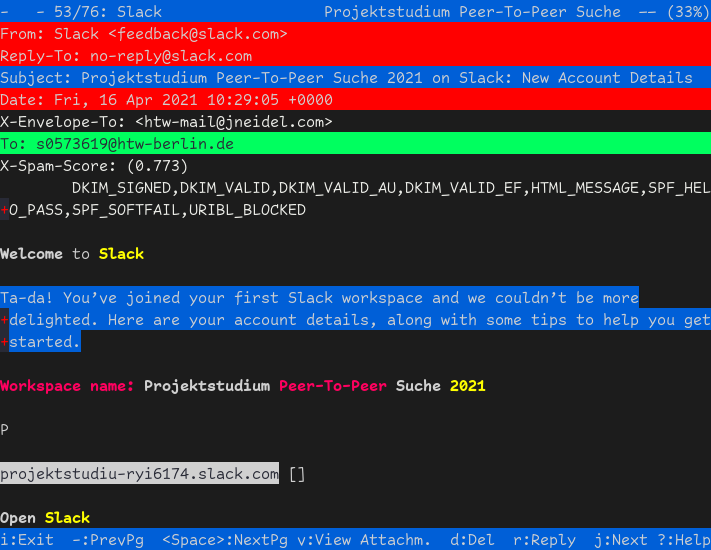
\includegraphics[scale=.47]{menu-example.png}
  \caption{Beispiel eines TUI: Emails im Terminal mit \codeinline{neomutt}.}
  \label{fig:menu-example}
\end{figure}

Laut \textcite{Paap_1988} wandelt das Menü das Problem des
\hyperref[prob:cr]{`Command Recall'} in `Command
Recognition', ein Wiedererkennen, um. Auch werden die Anfälligkeit für
\hyperref[prob:ss]{Syntaxfehler} reduziert, weil der Nutzer vor
illegalen Optionen abgeschirmt wird \parencite{Kantorowitz_1989}.

Im einem vergleichenden Experiment mit der Kommandozeile stellte
\textcite{Westerman_1997} für manche Nutzergruppen unsignifikant bessere Performance
fest. Auch wurde bei freier Wahl das Menü über alle Nutzergruppen hinweg doppelt
so häufig zur Nutzung ausgewählt.

Verglichen mit dem GUI sind TUI's trotzdem für Anfänger trotzdem schlechter
(in Performance und Meinung). Bei Experten liegen beide gleichauf
\parencite{tuivsgui}.

\subsubsection{Interaktive CLI}
\label{sec:def-interactive}

\begin{figure}[H]
  \centering
  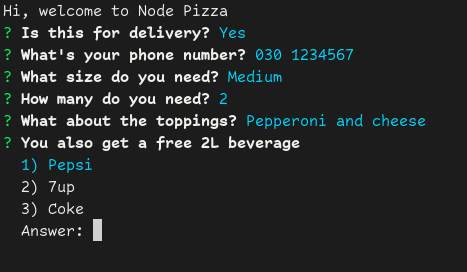
\includegraphics[scale=0.5]{interactive-example.png}
  \caption{Ein Interaktives CLI leitet durch eine Pizza Bestellung.}
  \label{fig:interactive-example}
\end{figure}

Das Interaktive CLI basiert auf einem ``question and answer model''
\parencite[42]{Spolsky_2001}. Dem Nutzer werden kontinuierlich Fragen gestellt
auf dieser er antwortet (siehe Abbildung \ref{fig:interactive-example}.) Durch
die hilfreichen Fragen entfällt der Bedarf sich an Kommandos erinnern zu müssen
(vgl. \hyperref[prob:cr]{`Command Recall'}.)

Je nach Bedarf kann der Nutzer nach einfachem Text-Input oder Zahlen
gefragt werden. Auch komplexeres, wie das Auswählen aus einer
Liste oder `multiple-choice` Fragen sind möglich (vgl. Abbildung
\ref{fig:interactive-example2}.)

\begin{figure}[H]
  \centering
  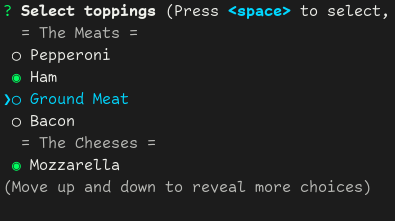
\includegraphics[scale=0.5]{interactive-example2.png}
  \caption{Der Belag einer Pizza wird interaktiv zusammengestellt.}
  \label{fig:interactive-example2}
\end{figure}

\subsection{Außerhalb des Terminals}
\label{sec:weiterentwicklung-ausser}

Historisch wurde die grafische Benutzeroberfläche als Lösung für die Probleme
des CLI gesehen (vgl. Kap. \ref{sec:historic-context}.) So wurden dem Nutzer die
möglichen Optionen grafisch präsentiert, anstatt diese nachschauen zu müssen.
(vgl. \hyperref[prob:cr]{`Command Recall'}.)

Es vollzog sich damit ein Wechsel von der funktionsorientierten
Kommandozeile hin zum objektorientierten GUI \parencite{nielson1993}. Die
Funktionsorientiertheit drückt sich etwa durch die in `single-command' CLI Apps
häufig vertretene Verb-Nomen Struktur aus. Beispielsweise in \codeinline{rm
FILE} oder \codeinline{cat FILE}. In der objektorientierten Welt gehen alle
Aktionen vom Objekt aus. So wird eine Datei in den Papierkorb gezogen (vgl.
\codeinline{rm FILE}) oder per Doppelklick angezeigt (vgl. \codeinline{cat
FILE}). Semantische Probleme (wie mit \codeinline{mv} die Reihenfolge
durcheinander zu bringen) sind damit passé. Und von der Textform befreit, sind
es auch die in der Kommandozeile prävalenten \hyperref[prob:ss]{Syntaxfehler}.

Aber auch das grafische User Interface hat seine Schwächen. Und diese werden vor
allem `at scale' sichtbar. Die Massen des Internets lassen sich nicht grafisch
darstellen und auch ein volles Email Postfach ist mit nur grafischen Werkzeugen
wenig durchsichtig. \textcite{Norman_2007} beschreibt wie Suchmaschinen hier einen
Ausweg bieten. Und nennt sie `answer engine'. Eine flexiblere, robustere und
getarnte Kommandozeile die mit Rechtschreibfehlern und Synonymen umgehen kann.

\chapter{Entwicklung von Methoden}
\label{sec:methods}
% TODO: intro here
% Methoden beziehen sich direkt auf ein Problem welches adressiert werden soll.

\section{Methodologie}

Nach Betrachtung der \hyperref[sec:cli-problems]{Probleme} sollten in
Literaturrecherche Lösungsansätze erarbeitet werden, welche zusammen mit einer
Erklärung als Methoden formuliert wurden.

Auf der Abstraktionsskala von Softwarekonzepten befindet sich die Methode in der
Mitte zwischen abstrakt und konkret.

\begin{code}
  \begin{shellcode}
abstrakt <-----------------------> konkret
   Prinzip <---> Methode <---> Werkzeug
  \end{shellcode}
  \captionof{listing}{Abstraktionsskala von Softwarekonzepten.}
  \medskip
\end{code}

Das abstrakte und allgemeine Prinzip \parencite{Balzert_2009} wäre zu
philosophischer Natur gewesen um im nächsten Schritt angewandt zu werden.
Werkzeuge nach \textcite{Balzert_2009} sind zu konkret und real. Es nicht Ziel
für jeden Lösungsansatz ein direkt anwendbares Werkzeug zu kreieren.

Eine Methode nach \textcite{Balzert_2009} ist eine begründete Vorgehensweise zur
Erreichung festgelegter Ziele. Sie ist nicht deskriptiv wie ein Werkzeug, und
nicht philosophisch wie ein Prinzip, sondern gibt eine Handlungsanweisung die
dem Entwickler Spielraum in der Implementierung lässt.

Die zu formulierenden Methoden sollten sich daher: auf Probleme die durch sie
gelöst/gemindert werden beziehen. Und begründet darstellen, warum dieser Effekt
eintreten wird.

Nachfolgend nun die erarbeiteten Methoden.

% TODO: unterliegende philosophie/prinzipien hier

\newcounter{meth}
\newcommand{\methbox}[2]{
  \medskip
  \medskip
  \fbox{\parbox{\linewidth}{
    \refstepcounter{meth}
    \textbf{Methode~\themeth}: #2
    \label{meth:#1}
  }}
  \medskip
}
\newcommand{\methref}[1]{
  Methode~\ref{meth:#1}
}

\section{Flaggen anstatt Argumenten}

Sobald ein (Sub-) Kommando mehr als ein Argument annimmt, bietet sich die
Gelegenheit, die für Argumente relevante Reihenfolge durcheinander zu bringen
(vgl. \refss{Syntax/Semantik}.) \textcite{12factor} empfiehlt deshalb bei
zwei oder mehr Argumenten anstatt dieser Flaggen zu verwenden. Das ist etwas
mehr Aufwand zum Schreiben, eliminiert aber die Reihenfolge als Fehlerfaktor.
Außerdem können Flaggen auch mittels Autovervollständigung vorgeschlagen werden
(vgl.~\methref{autocomplete}).

\methbox{flags_over_arguments}{Verwende Flaggen, wenn mehr als ein Argument benötigt wird.}

Dies trifft vor allem zu wenn ein (Sub-) Kommando gleichzeitig Parameter über
Flaggen und Argumente entgegennimmt.

\begin{code}
  \begin{shellcode}
# Argument und Flaggen Kombination
$ oraclett project add INTPD999DXD --taskDetail "01 - Career development"

# Nur Flaggen
$ oraclett project add --project INTPD999DXD --taskDetail "01 - Career development"
  \end{shellcode}
  \captionof{listing}{Argument ersetzt durch Flaggen: vorher und nachher}
  \medskip
\end{code}

Außen vor sind Kommandos welche eine variable Anzahl von Argumenten annehmen.
Beispielsweise \codeinline{rm} dem mehrere Dateien zum Löschen übergeben
werden können. Hier handelt es sich aber nicht um Argumente mit verschiedenen
Bedeutungen (\textcite{12factor}.)

Ein weiter Vorteil ist das Erstellen von Aliasen zu vereinfachen. Das sind
Abkürzungen, die ein Nutzer sich innerhalb seiner Shell definieren kann. Etwa um
ein Kommando abzukürzen: \codeinline{alias v="nvim"} macht \codeinline{nvim} mit
dem Kommando \codeinline{v} nutzbar.

Man stelle sich vor eine CLI App nimmt ein eine Anzahl von Stunden und ein Datum:

\begin{code}
  \begin{shellcode}
$ app HOURS DATE
  \end{shellcode}
\end{code}

Der Nutzer möchte einen Alias mit dem für den heutigen Tag eine Anzahl von Stunden übergeben wird.
Gewünschte Nutzung des Alias sieht so aus:

\begin{code}
  \begin{shellcode}
$ apptoday 8
  \end{shellcode}
\end{code}

Um diesen Alias zu ermögliche muss aber eine kompliziertere\footnote{Neulinge
kommen mit der Alias Syntax meist früher in Kontakt. Neben unvertrauter Syntax
spielt mit hinein das Shell Argumente (\codeinlinefn{\$1}) verwendet werden müssen und das die
Möglichkeit entfällt dynamisch weitere Flaggen zu übergeben.} Shell Funktion
definiert werden, weil das Argument an die richtige Stelle übergeben werden
muss:

\begin{code}
  \begin{shellcode}
apptoday() {
  app $1 today
}
  \end{shellcode}
\end{code}

Würde \codeinline{app} anstatt der Argumente Flaggen annehmen:

\begin{code}
  \begin{shellcode}
$ app --hour HOURS --date DATE
  \end{shellcode}
\end{code}

Dann wäre der Alias viel leichter und flexibler zu definieren:

\begin{code}
  \begin{shellcode}
$ alias apptoday="app --date today --hour"
  \end{shellcode}
\end{code}

Wenn die Stunde anstatt des Tages durch den Alias festgeschrieben werden soll,
ist das mit der Flaggen-basierten Struktur auch kein Problem. Der Nutzer ist
unabhängig von der durch den Entwickler definierten Reihenfolge.

\section{Unterstützung aller Hilfs- und Versionsflaggen}

Der Großteil aller Apps bietet eine Hilfs- und eine Versionsseite. Hilfsseiten
beschreiben ähnlich wie eine `man page'\footnote{Einer über das \codeinlinefn{man}
Kommando verfügbaren Hilfsseite.} die Subkommandos, Flaggen und Syntax. Meist
sind diese auch relativ und beziehen sich auf das aktuelle Subkommando.
Versionsseiten geben die Version der App\footnote{Sowie ggf. eine Liste von
optionalen Features die mit einkompiliert wurden.} wieder.

\begin{code}
  \begin{shellcode}
$ mullvad status --help
mullvad-status
View the state of the VPN tunnel

USAGE:
    mullvad status [OPTIONS] [SUBCOMMAND]

OPTIONS:
        --debug       Enables debug output
    -h, --help        Print help information
    -l, --location    Prints the current location and IP. Based on GeoIP lookups
    -v                Enables verbose output

SUBCOMMANDS:
    listen    Listen for VPN tunnel state changes
  \end{shellcode}
  \captionof{listing}{Als Beispiel: Die gekürzte, relative Hilfsseite von \codeinline{mullvad status}.}
  \medskip
\end{code}

Beim Aufrufen dieser Seiten haben Nutzer ihre Präferenzen wenn es darum geht
welche Flagge sie verwenden um diese angezeigt zu bekommen.

\begin{code}
  \begin{shellcode}
$ app -h
$ app --help
$ app help

$ app -v
$ app -V
$ app --version
$ app -version
\$ app version
  \end{shellcode}
  \captionof{listing}{Gängige Varianten der Hilfs- und Versionsflaggen.}
  \medskip
\end{code}

Laut \textcite{12factor} sollten möglichst alle Varianten in von einer Anwendung
unterstützt werden. So kann vermieden werden, dass der Nutzer nicht das
angezeigt bekommt, wonach er sucht. Das Problem des \refcrr wird vermieden, weil
der Nutzer durch Probieren seiner präferierten Variante direkt zur Lösung kommt.

\methbox{support_all_help_version}{Unterstütze alle gängigen Formen der Hilfs- und Versionsflaggen.}

\newcommand\checkmark{\ttfamily{\char"2611}}
\newcommand\cross{\ttfamily{\char"2610}}
\begin{table}[h!]
  \begin{center}
    \label{tab:help_version}
    \begin{tabular}{l | c c c | c c c c c}
      Kommando & \codeinline{-h} & \codeinline{--help} & \codeinline{help} & \codeinline{-v} & \codeinline{-V} & \codeinline{--version} & \codeinline{-version} & \codeinline{version} \\
      \hline
git & \checkmark & \checkmark & \checkmark & \checkmark & \cross & \checkmark & \cross & \checkmark\\
node & \checkmark & \checkmark & \cross & \checkmark & \cross & \checkmark & \cross & \cross\\
mullvad & \checkmark & \checkmark & \cross & \cross & \cross & \cross & \cross & \checkmark\\
grep & \cross & \checkmark & \cross & \cross & \checkmark & \checkmark & \cross & \cross\\
zathura & \checkmark & \checkmark & \cross & \checkmark & \cross & \checkmark & \cross & \cross\\
tsp & \checkmark & \cross & \cross & \cross & \checkmark & \cross & \cross & \cross\\
pubs & \checkmark & \checkmark & \cross & \checkmark & \cross & \checkmark & \cross & \cross\\
ffmpeg & \checkmark & \checkmark & \cross & \cross & \cross & \cross & \checkmark & \cross\\
systemctl & \checkmark & \checkmark & \cross & \cross & \cross & \checkmark & \cross & \cross\\
pacman & \checkmark & \checkmark & \cross & \cross & \checkmark & \checkmark & \cross & \cross\\
make & \checkmark & \checkmark & \cross & \checkmark & \cross & \checkmark & \checkmark & \cross\\
synctex & \checkmark & \checkmark & \checkmark & \checkmark & \checkmark & \checkmark & \checkmark & \checkmark\\
curl & \checkmark & \checkmark & \cross & \cross & \checkmark & \checkmark & \cross & \cross\\
ansible & \checkmark & \checkmark & \checkmark & \cross & \cross & \checkmark & \cross & \cross\\
nvim & \checkmark & \checkmark & \cross & \checkmark & \cross & \checkmark & \checkmark & \cross\\
      \hline
      Summe & 14 & 14 & 3 & 7 & 5 & 12 & 4 & 3 \\
    \end{tabular}
    \caption{Unterstützte Varianten von Hilfs- und Versionsflaggen bei einer Stichprobe von 15 Kommandos.}
  \end{center}
\end{table}

In einer unrepresentativen Stichprobe (siehe Tabelle) wurde zusammengestellt,
welche Flaggen in 15 Anwendungen funktionieren bzw. nicht funktionieren. Dabei
stellte sich heraus, dass \codeinline{-h} und \codeinline{--help} praktisch
überall funktionieren. Mit \codeinline{--version} wird in den meisten Fällen
auch das gewünschte Ergebnis angezeigt. Aber wenn \codeinline{--version} nicht
zum Ziel führt ist durchprobieren angesagt.

Am wenigsten verbreitet sind \codeinline{help} und \codeinline{version},
welche aber auch etwas außen vor sind, weil das erste Argument bei vielen
`single-command' Kommandos eine `Input' Datei bezeichnet. Aber bei
`multi-command' Apps sollten auch diese Varianten unterstützt werden.

\section{Relevante Standardwerte}

Relevante `Defaults' sind nicht Kommandozeilen-spezifisch, können dort aber
wichtiger sein als in grafischen Anwendungen.

Dem Nutzer werden die Möglichkeiten eben nicht zur Auswahl gestellt und dieser
klickt die gewünschte Option an. Sondern ist das Auflisten der Möglichkeiten
i.d.R. ein separater Schritt, losgelöst von der eigentlich beabsichtigten
Aktion. Beispielsweise muss um sich mit \codeinline{cd} in einen Ordner
hineinzubewegen der Name dessen zuerst in Erfahrung gebracht werden (etwa mit
\codeinline{ls -d}.)

Es greift wieder das fundamentale Problem des \refcrr. Den Schritt des
Auflistens der Möglichkeiten (ähnlich wie das Auflisten von möglichen Kommandos)
ist ein extra Schritt der nur nötig ist weil der Nutzer sich nicht an die Option
erinnern kann die er verwenden möchte.

\bigskip

\methbox{relevant_defaults}{Biete relevante Standardwerte an.}

Dem Nutzer relevante Defaults anzubieten erlaubt es diesem weniger Argumente an
die CLI App übergeben zu müssen. Es gibt weniger Fehlermeldungen die den Nutzer
zurückweisen, weil dieser etwas vergessen hat.

Es ist aber auch elementar die Nutzung dieser Standardwerte zu kommunizieren.
Damit der Nutzer von ihnen nicht überrascht wird.

\section{Interaktives Nachfragen bei fehlendem Parameter}

Man stelle sich folgendes Szenario vor. Eine CLI App hat ein Subkommando welches
einen Parameter erfordert. Normalerweise erfolgt bei nicht-Übergabe dieses
Parameters eine Fehlermeldung welche darauf hinweist.

\begin{code}
  \begin{shellcode}
$ mullvad relay set location
error: The following required arguments were not provided:
    <country>

USAGE:
    mullvad relay set location <country> [ARGS]

For more information try --help
  \end{shellcode}
  \captionof{listing}{Fehlermeldung bei fehlendem Parameter in \codeinline{mullvad}'s CLI.}
  \label{lst:missing-param}
  \medskip
\end{code}

Die Anwendung weiß aber bereits was der Nutzer tun möchte und könnte anstatt
der Fehlermeldung dem Nutzer mit einer Eingabeaufforderung (interaktivem
Nachfragen, vgl. Kapitel \ref{sec:def-interactive}) nach dem fehlenden
Parameter fragen \parencite{12factor}. Oder, je nach Kontext, diesem sogar
eine Liste von Vorschlägen geben, um daraus auswählen. Dem Nutzer wird erspart
sich damit auseinander zu setzen welche Parameter erfordert sind (vgl.
\hyperref[prob:cr]{`Command Recall'})

\methbox{interactive_missing_param}{Frage bei fehlendem Parameter interaktiv nach.}

\begin{code}
  \begin{shellcode}
$ mullvad relay set location
Enter location country code:
  \end{shellcode}
  \captionof{listing}{Beispiel der Eingabeaufforderung zur Verbesserung von Listing \ref{lst:missing-param}.}
  \medskip
\end{code}

Fairerweise ist zu bemerken das die mullvad CLI App dies auch, an anderer Stelle,
genau so handhabt. Bei \codeinline{mullvad account login} wird nach der
fehlenden Accountnummer gefragt.

Mit einer Fehlermeldung anstatt des interaktivem Nachfragens könnte der
Nutzer leichter auf die ggf. komplexere Verwendung des Kommandos hingewiesen
werden. So nimmt das mullvad Kommando aus dem ersten Beispiel neben der
Landeskennung auch noch optional die ein Stadt- und `Hostkennung'. Was aber
aus der Fehlermeldung auch nicht klar hervorgeht. Wenn unter Berücksichtigung
dieser Methode implementiert wird kann dieser Einwand aber auch mitigiert
werden. Entweder durch das Vereinfachen oder Umgestalten der Kommandos. Oder mit
Hinweisen auf die Hilfsseite, welche die Parameter vollumfänglich erklärt.

\section{Natürliche Sprache}
\label{sec:natural-lang}

\textcite{Raskin_2008} beschreibt die Kapazitäten linguistischer
Kommandozeilen, welche Normans Konzept der `answer engines' (vgl. Kapitel
\ref{sec:weiterentwicklung-ausser}) ähneln. Diese haben wie der Name schon
hergibt einen Fokus auf menschlicher Sprache\footnote{Die Linguistik ist das
Studium der menschlichen Sprache.}. Ein schönes, genanntes Beispiel von Google
Calendar für die Stärke solcher, auf natürlicher Sprache basierender Interfaces:
``Sunday dinner at 7:30 p.m. with Asa Jasa.'' Es werden keine Kommandos
verwendet. Das gewünschte wird einfach in natürlicher Sprache beschrieben.
Syntax ist nur insofern relevant, als das die menschliche Sprache ihre eigene
Syntax hat.

``Recently, there has been a growing movement that sees today's command line
as a human-first text-based UI, rather than a machine-first scripting platform
\parencite{clig}'' - \parencite{Schr_der_2021}

Die Syntax- und Semantikeinschränkungen des Kommandozeilen-Interfaces lassen
eine alleinig `human language'-gestützte Anwendung nicht zu. Zumindest nicht
der Reinform des CLI. Als `human-first` User Interface sollte trotzdem
zumindest eine eingschränkte Form natürlicher Spracheingabe unterstützt werden
\parencite{seneviratne2008new}.

\methbox{human_language}{Unterstütze Eingaben in natürlicher Sprache.}

\section{Fehlerkorrektur}

Diese Methode zeigt eine gewisse Nähe zur Unterstützung der natürlichen
Sprache (Kapitel \ref{sec:natural-lang}). So hob \textcite{Raskin_2008} für die
linguistische Kommandozeile die Verträglichkeit von Rechtschreibfehlern hervor.

Fehlertoleranz im Bezug auf Rechtschreibung würde auch das Problem der zu
\refss{strikten Syntax} zum Teil adressieren. Fehlermeldungen und die damit
einhergehende Frustration minimieren. \textcite{clig} empfehlen ganz konkret: ``If
the user did something wrong and you can guess what they meant, suggest it.''
Im Kontrast dazu soll nach der `Do what I mean' Philosophie der Fehler direkt
und ohne Nutzerfeedback ausgebessert werden \parencite{DWIM}. Was natürlich
schneller ist und den Nutzungsflow nicht unnötig unterbricht. \textcite{clig} weisen
aber auch darauf hin das eine fehlerhafte Eingabe neben Rechtschreibfehlern eben
auch aus logischen Fehler resultieren kann. Dann kann `Do what I mean' zu sehr
unerwartetem, gefährlichem Verhalten führen.

\methbox{typos}{Unterstütze (suggestive) Fehlerkorrektur.}

\begin{code}
  \begin{shellcode}
heroku pss
 ›   Warning: pss is not a heroku command.
Did you mean ps? [Y/n]:
  \end{shellcode}
  \captionof{listing}{Korrekturvorschlag eines Rechtschreibfehlers nach \textcite{clig}.}
  \medskip
\end{code}

\section{Autovervollständigung}

`Auto-completion' in der Kommandozeile beschreibt das beim Drücken der `TAB' Taste
etwas ergänzt/vervollständigt wird.

In der Shell funktioniert dies etwa für Kommandos und Dateipfade:
\begin{code}
  \begin{shellcode}
$ wg # Nutzer drückt TAB
$ wget

$ cat ./note # Nutzer drückt TAB
$ cat ./notes.md
  \end{shellcode}
  \captionof{listing}{Autovervollständigung in der Shell.}
  \medskip
\end{code}

Innerhalb einer CLI App kann die Vervollständigung, neben Dateipfaden, auch
Subkommandos und Flaggen umfassen.

\begin{figure}[H]
  \centering
  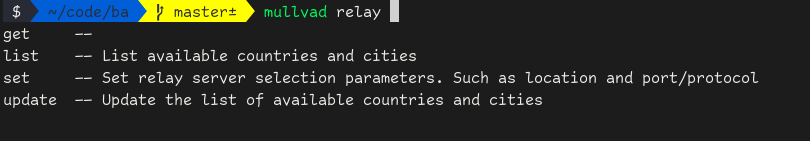
\includegraphics[scale=0.5]{mullvad-autocomplete.png}
  \caption{\codeinline{mullvad}'s CLI listet nach dem drücken von `TAB' mögliche Subkommandos.}
  \label{fig:autocomplete}
\end{figure}

`Auto-completion' adressierte beide Probleme welche das CLI mit sich bringt.
Durch das Vorschlagen und Vervollständigen wird das \refcr{Erinnern}
erleichtert. Und dadurch das nur valide Kommandos vorgeschlagen werden ist das
einhalten von \refss{Syntax- und Semantikregeln} erleichtert. Auch profitiert
der Nutzer von Kontext-bezogenen Beschreibungen.

\methbox{autocomplete}{Nutze Autovervollständigung zum Vorschlagen von Flaggen
und Subkommandos \parencite{seneviratne2008new}.}

In \textcite{dutta} geht der Author sogar noch einen Schritt weiter und empfiehlt
das automatische Vorschlagen aller Flaggen und Argumente für ein Kommando,
sodass der Nutzer sich nicht mal anschauen muss was für das Kommando benötigt
wird. So wie vom Author beschrieben ist dies aber nicht in der Shell möglich,
sondern müsste in einer eigenen Kommandozeilen Umgebung umgesetzt werden.

\section{Menü-basiertes Interface}

Im Kapitel \ref{sec:def-menu} wurde schon darauf eingegangen wie ein
TUI die Probleme der Kommandozeile adressieren würde. Auch wurde eine
klare Präferenz für ein solches Interface unter den Nutzern festgestellt
\parencite{Westerman_1997}. Auch \textcite{Spolsky_2001} nennt das Menü-basierte
Interface als einen Weg Usability zu erhöhen.

\methbox{menu}{Biete ein Menü-Interface an.}

\section{Relevante Kommandovorschläge}

Die Essenz von \refcrr ist das Nutzer nicht wissen welche (Sub-) Kommandos
ihnen zur Verfügung stehen. Kommandos existieren aber nicht im Vakuum. Im
Zusammenspiel unterliegen sie meist einer gewissen Reihenfolge bzw. einem
`Nutzungsflow'. Bevor in einen Ordner gewechselt werden kann (\codeinline{cd})
muss dieser erst existieren (\codeinline{mkdir}) oder der Nutzer muss um diesem
wissen (\codeinline{ls}). \textcite{dutta} schlägt nun vor sich diesen `Flow'
zu nutze zu machen um den Nutzer über mögliche nächste Schritte (in Form
anderer (Sub-) Kommandos) zu informieren. Für den gegebenen `Flow' könnte
also \codeinline{mkdir} mit einer Nachricht à la \codeinline{Also look at -
cd, ls} versehen werden. Diese Vorschläge können als Erinnerung dienen oder
den Nutzer dazu Auffordern sich die Vorschläge einmal näher anzuschauen. Bei
`multi-command' CLI Apps mit vielen Subkommandos, wo der Nutzer nicht weiß wo er
anfangen soll, sind diese Vorschläge besonders wertvoll.

\methbox{command_recommendations}{Schlage dem Nutzer andere relevante
Subkommandos vor \parencite{seneviratne2008new}.}

\chapter{Beispiel Anwendung}
\label{sec:beispiel-anwendung}

\section{Anforderungsanalyse}

Die zu bauende Anwendung wurde so konzipiert das diese weder zu trivial noch
zu komplex ist. Nicht zu trivial damit das Interface auch wirklich etwas
leisten muss und nicht zu simpel sein kann. Aber auch nicht zu komplex um die
Umsetzbarkeit innerhalb des Zeitrahmens zu gewährleisten.

\subsection{Konzept}

Bei Endava\footnote{Der Firma in welcher diese Bachelorarbeit geschrieben
wurde.} werden die Arbeitsstunden über eine interne Webapp (ein Oracle System)
festgehalten. Diese Webapp wird im Laufe der Arbeit als \textbf{Oracle}
bezeichnet\footnote{Unter diesem Namen ist das System auch firmenintern
bekannt.}.

\begin{figure}[H]
  \centering
  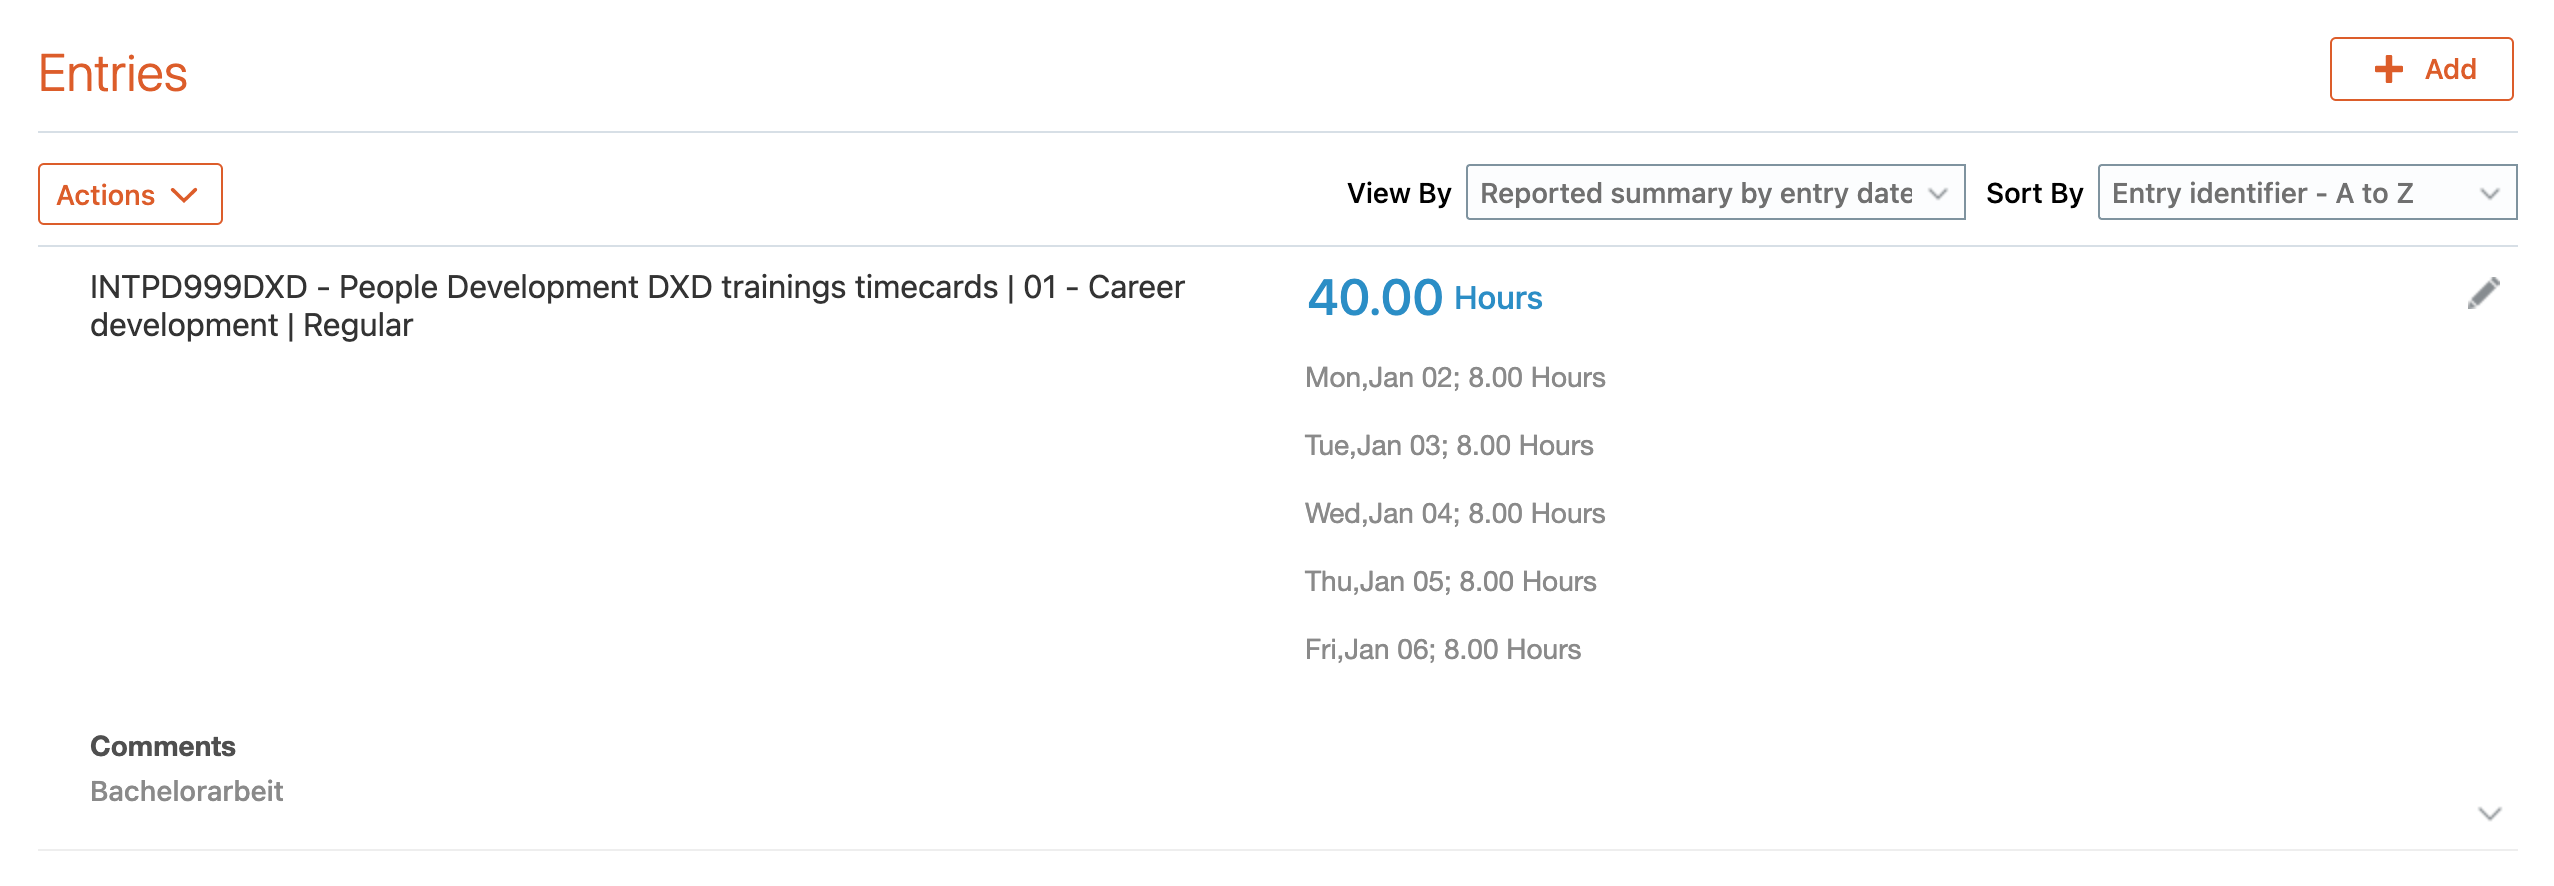
\includegraphics[scale=0.25]{oracle-ideal.png}
  \caption{Idealtypische Oracle `Timecard'.}
\end{figure}

Am Ende der Arbeitswoche werden die Arbeitsstunden der vergangen Woche in
einer sogenannten `Timecard' festgehalten. Dabei wird angegeben an welchen
Wochtage wieviele Stunden an welchen Projekten gearbeitet wurde. Wenn nur an
einem einzigen Projekt mit gleichbleibenden 40 Stundenwoche gearbeitet wird ist
dieser Prozess trivial. Wenn man aber als Werkstudent an mehreren Projekten mit
schwankenden Stundenzahlen arbeitet wird es schnell komplizierter. Und wenn dazu
noch dokumentiert werden soll woran gearbeitet wurde noch umso mehr. Dies heißt
praktisch das die ‘Timecard’ täglich in Oracle aktualisiert werden muss.

\begin{figure}[H]
  \centering
  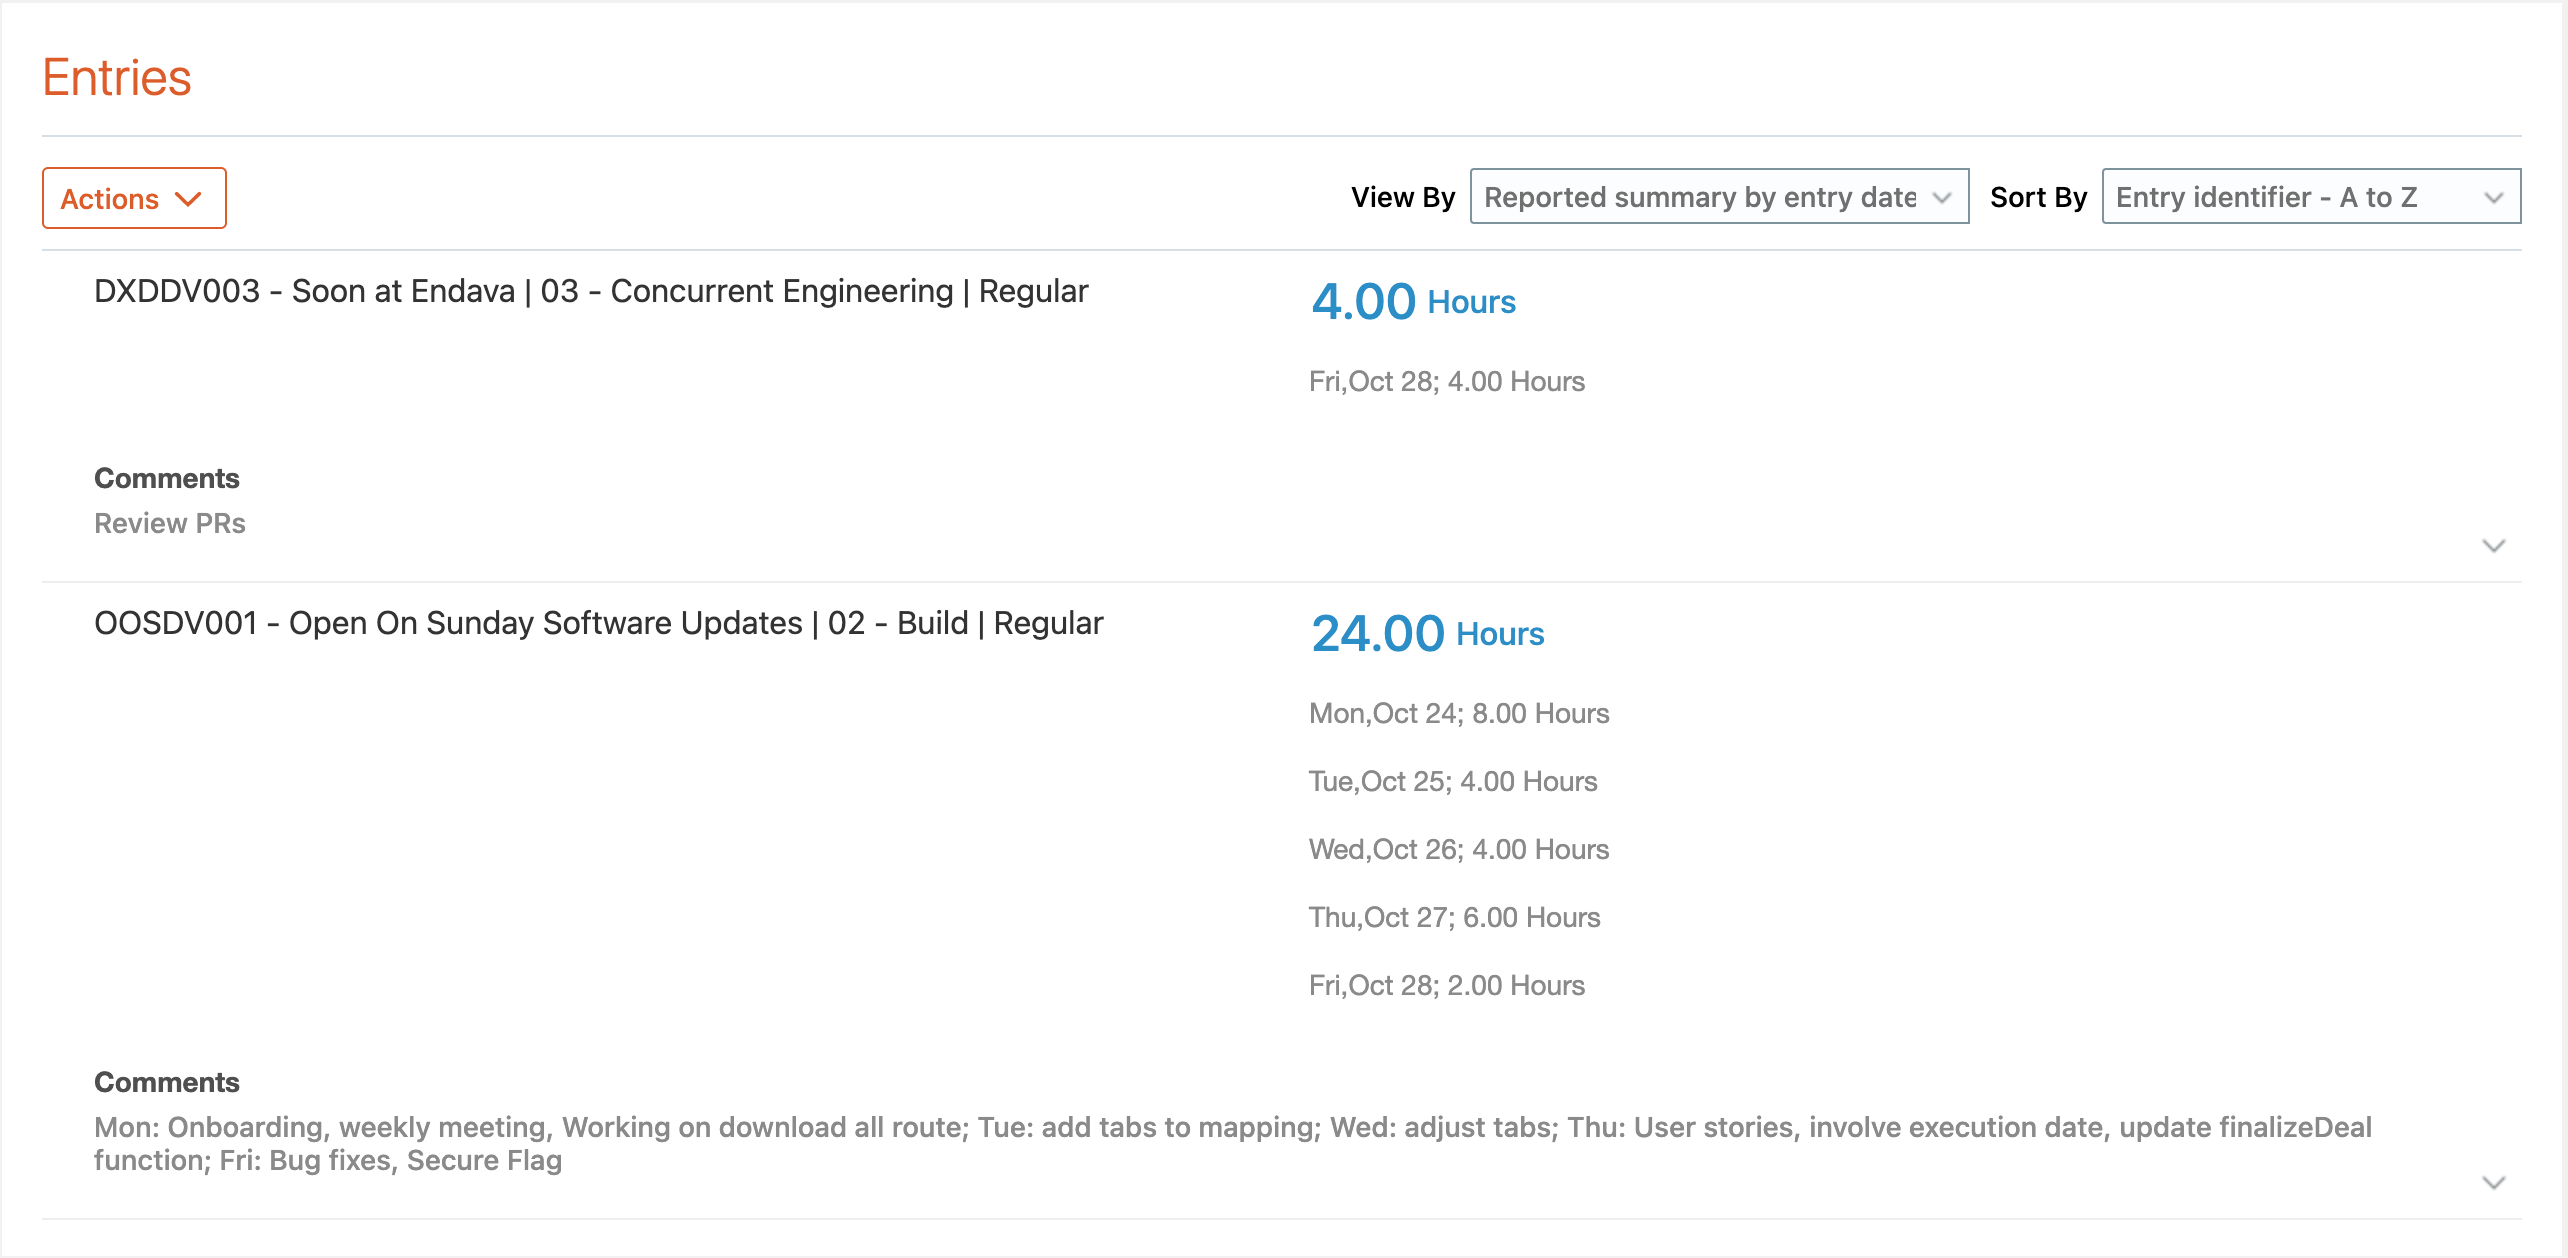
\includegraphics[scale=0.25]{oracle-real.png}
  \caption{Eine weniger idealtypische `Timecard'.}
\end{figure}

Um eine Alternative zur Webapp zu schaffen wurde eine Kommandozeilen App
entworfen, welche praktisch die gleichen Kapazitäten anbietet. Es können täglich
die Arbeitszeiten sowie Notizen dazu woran gearbeitet wurde festgehalten
werden. Um eine sinnvolle Alternative darzustellen sind auch die Kapazitäten
zum Verwalten von Projekten und dem Übertragen der Daten zu Oracle notwendig
\footnote{Eine mögliche, direkte Übertragung an Oracle selbst würde den Rahmen
der Arbeit sprengen, ohne dem Thema dienlich zu sein. Weshalb davon abgesehen
wurde.}. Ohne Projektverwaltung würde die Zuordnung erschwert. Und ohne explizit
unterstütztes Übertragen wäre die Anwendung weit weniger hilfreich.

\subsection{Anforderungen}

Die Anforderungen wurden in Form von User Stories festgehalten. Erhoben wurden
diese durch den Author in Analyse der eigenen Nutzungsmuster mit Oracle,
abgeglichen in Rücksprache mit anderen Mitarbeitern.

\begin{enumerate}
  \item \textbf{Projekte}:
    \begin{enumerate}
      \item Als Nutzer möchte ich ein Projekt hinzufügen.
      \item Als Nutzer möchte ich einem Projekt einen oder mehrere Task Details anfügen.
      \item Als Nutzer möchte ich die Projekte sowie deren Task Details aufgelistet sehen.
      \item Als Nutzer möchte ich Projekte und Task Details anpassen oder löschen können.
    \end{enumerate}
  \item \textbf{Arbeitszeit}:
    \begin{enumerate}
      \item Als Nutzer möchte ich meine Arbeitsstunden an einem Tag für eine Projekt-Task Detail Kombination loggen.
      \item Als Nutzer möchte ich die geloggten Arbeitsstunden einer gegebenen Woche einsehen.
      \item Als Nutzer möchte ich geloggte Arbeitsstunden anpassen oder löschen können.
    \end{enumerate}
  \item \textbf{Arbeitsnotizen}:
    \begin{enumerate}
      \item Als Nutzer möchte ich festhalten woran ich gearbeitet habe.
      \item Als Nutzer möchte ich meine Notizen sehen können.
      \item Als Nutzer möchte ich meine Notizen bearbeiten oder löschen können.
    \end{enumerate}
  \item \textbf{Timecard}:
    \begin{enumerate}
      \item Als Nutzer möchte ich die Daten für die Timecard zu einer gegebene Arbeitswoche sehen, um diese nach Oracle zu übertragen.
    \end{enumerate}
\end{enumerate}

Diese User Stories sollen einen Eindruck über die Anforderungen der App
und deren Komplexität vermitteln. Das Bauen der App steht aber nicht im
Vordergrund, weshalb hier u.a. die Akzeptanzkriterien der User Stories,
Implementationsdetails wie Datenpersistierung, etc. nicht weiter beschrieben
werden.

\section{Technische Aspekte}
\subsection{Fundament}

Das Fundament der App stellen die zugrundelegenden technologischen Aspekte dar,
welche nicht oder nur indirekt die Nutzbarkeit, und damit den Fokus der Arbeit
betreffen.

Node.js wurde als Programmiersprache gewählt, weil der Author damit vertraut
war, eine Vielzahl von Libraries zum Bauen von CLI Apps existieren und der
Paketveröffentlichungsprozess mit npm relativ simpel ist. Weiterhin wurden noch
Typescript - für Typisierung - und Eslint - für gleichmäßigen Code Style -
verwendet.

\subsection{Libraries}

Ein Überblick über die Libraries welche für das Bauen des Interfaces und die
Umsetzung der Methoden relevant waren.

\subsubsection{oclif}
\label{sec:oclif}

``oclif is an open source framework for building a command line interface
(CLI) in Node.js. Create CLIs with a few flags or advanced CLIs that have
subcommands.'' - \textcite{oclif}

Mit oclif können problemlos `multi-command' App gebaut werden. Die Hierarchie
der Subkommandos wird über die Dateistruktur angegeben:

\begin{code}
  \begin{shellcode}
 src/commands
 └── project
     ├── add.ts
     ├── edit.ts
     ├── list.ts
     └── remove.ts
  \end{shellcode}
  \captionof{listing}{Subkommandohierarchie am Beispiel des \codeinline{project} Subkommandos.}
  \medskip
\end{code}

In einer dieser Dateien können nun ohne viel Boilerplate die Flaggen,
Argumente und Beschreibung und spezfiziert werden. Danach wird nur noch die
eigene Businesslogik angeschlossen (siehe Abbildung \ref{fig:oclif-list} für
ein Implementationsbeispiel.) oclif übernimmt dabei das Subkommando- und
Flaggenparsing, generiert die Hilfseite, uvm.

\begin{figure}[H]
  \centering
  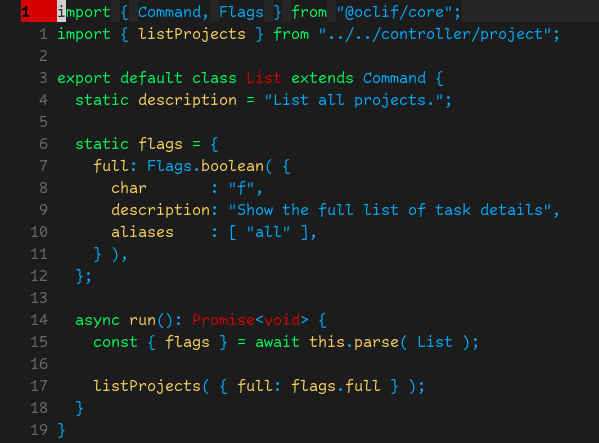
\includegraphics[scale=0.62]{oclif-list.png}
  \caption{Implementation des \codeinline{project list} Subkommandos.}
  \label{fig:oclif-list}
\end{figure}

Der Feinschliff wird noch per Konfiguration in der \codeinline{package.json}
erreicht. oclif kümmert sich dabei um die Kleinigkeiten. Zum Beispiel wird
sichergestellt das der Text der Hilfsseiten richtig formatiert wird. Im
unterstehenden Listing wird demonstriert wie oclif bei eingeschränkter Breite
des Terminals den Text so einrückt, dass immer noch klar zu erkennen ist was
Beschreibung und was Flagge ist. Das Gegenbeispiel dazu entsteht wenn einfach
nur der Text auf den Bildschirm geschrieben wird, ohne die Terminalbreite zu
berücksichtigen.

\begin{code}
  \begin{shellcode}
# in oclif
FLAGS
  -d, --date=<value>  [default: today] A date to specify the day OR
                      the week (can be human-readable)

# ohne Framework
FLAGS
  -d, --date=<value>  [default: today] A date to specify the day OR
the week (can be human-readable)
  \end{shellcode}
  \captionof{listing}{oclif's Handhabung von Zeilenumbrüchen in einem schmalen Terminal im Vergleich zu einer Implementierung ohne Framework}
  \label{lst:oclif-umbruch}
  \medskip
\end{code}

\medskip

Neben oclif wurde noch andere Frameworks/Libraries in Erwägung gezogen. U.a.
\href{https://github.com/tj/commander.js}{commander.js},
\href{https://github.com/yargs/yargs}{yargs},
\href{https://github.com/dthree/vorpal}{vorpal} und
\href{https://github.com/sindresorhus/meow}{meow}.

\subsubsection{Inquirer.js}

Inquirer ist eine Ansammlung von interaktiven Fragetypen (vgl. Kapitel
\ref{sec:def-interactive}). Neben einfachen Fragen, wie Text einzugeben oder
einen Eintrag aus einer Liste auswählen, gibt es auch `multiple-choice' (siehe
Abb. \ref{fig:interactive-example2}) Fragen, das Bearbeiten von Text im
präferierten Texteditor, uvm.

\begin{figure}[H]
  \centering
  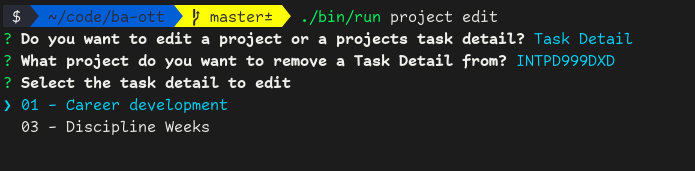
\includegraphics[scale=0.5]{inquirer-example.png}
  \caption{Ein Reihe von Fragen zum Herausfinden was der Nutzer bearbeiten möchte.}
  \label{fig:inquirer-example}
\end{figure}

\begin{code}
  \begin{javascriptcode}
const { whatToEdit } = await inquirer.prompt( [ {
  type   : "list",
  name   : "whatToEdit",
  message: "What do you want to edit?",
  choices: [
    {
      name : "Project Name",
      value: "project",
    },
    {
      name : "Task Details (of a project)",
      value: "taskDetail",
    },
  ],
} ] );

// wird zu:

? What do you want to edit? (Use arrow keys)
> Project Name
  Task Details (of a project)
  \end{javascriptcode}
  \captionof{listing}{Implementation für das Auswählen zwischen zwei Optionen.}
  \medskip
\end{code}

\section{Implementierte Anwendung}

Es folgt eine grobe Vorstellung der implementierten App. Es geht darum ein
Verständnis für den Kontext schaffen in welchem die Methoden implementiert
wurden. Diese werden dann im nächsten Schritt (im nächsten Kapitel) vorgestellt.

`oraclett' wurde als Name für die App gewählt. Der Name wurde in Anlehnung
an das interne Werkzeug zum Festhalten der Arbeitszeiten benannt (bekannt
als `Oracle') und steht für `Oracle time tracker'. Der Name sollte
1) kurz und prägnant als auch 2) mit Autovervollständigung leicht zu
vervollständigen sein. Mit \codeinline{oracle} beginnend ist die Assoziation
mit dem intern Tool hergestellt und kann beim drücken von TAB dann zu
\codeinline{oraclett} vervollständigt wird. Andere in Erwägung gezogene
Varianten waren \codeinline{oracle-time-tracker} oder \codeinline{ott}. Diese
waren aber zu lang bzw. kryptisch.

\begin{code}
  \begin{shellcode}
$ oraclett --help
Oracle time tracker

VERSION
  oraclett/0.1.1 linux-x64 node-v19.5.0

USAGE
  $ oraclett [COMMAND]

TOPICS
  hour      Log and manage hours.
  note      Write down and manage notes.
  project   Manage projects.
  timecard  Generate a report for filling out timecards.

COMMANDS
  help      Display help for oraclett.
  timecard  Generate a report for filling out timecards.
  \end{shellcode}
  \captionof{listing}{Das Hilfsmenu der CLI App.}
  \label{lst:oraclett-help}
  \medskip
\end{code}

\begin{code}
  \begin{shellcode}
$ oraclett hour --help
Log and manage hours.

USAGE
  $ oraclett hour COMMAND

COMMANDS
  hour add     Log working hours.
  hour edit    Edit the logged hours interactively.
  hour list    List all logged hours.
  hour remove  Remove logged hours interactively.
  \end{shellcode}
  \captionof{listing}{Hilfsseite des \codeinline{hour} Subkommandos}
  \label{lst:hour-help}
  \medskip
\end{code}

\label{text:noun-verb} Die Subkommandos sind nach dem `noun verb'
Prinzip \parencite{clig} strukturiert. Die Nomen sind dem ersten Listing
\ref{lst:oraclett-help} zu entnehmen: \codeinline{hour}, \codeinline{note},
\codeinline{project} und \codeinline{timecard}. Auf eines Nomen, im
obenstehenden Listing \ref{lst:hour-help} etwa die Stunde (\codeinline{hour}),
folgt ein Verb wie \codeinline{add}, \codeinline{edit}, \codeinline{remove}
oder \codeinline{list}. Diese Verben sind über alle Kommandos hinweg
einheitlich\footnote{Außer bei \codeinlinefn{timecard}, welches keine
Subkommandos hat.}. Zum Bearbeiten eines Projektes wird ebenso das Verb
\codeinline{edit} verwendet wie beim Bearbeiten einer Notiz.

Der vorgesehene Nutzungsflow wäre wie folgt. Wenn man einem neuen Projekt
zugewiesen wird fügt man dieses \codeinline{oraclett} mit \codeinline{project
add} hinzu.

\begin{figure}[H]
  \centering
  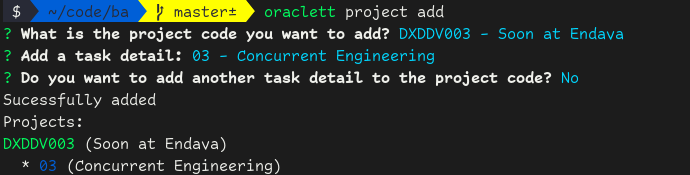
\includegraphics[scale=0.5]{project-add.png}
  \caption{Interaktives Hinzufügen von einem Projekt.}
  \label{fig:project-add}
\end{figure}

\begin{figure}[H]
  \centering
  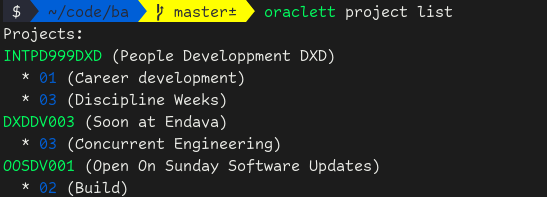
\includegraphics[scale=0.5]{project-list.png}
  \caption{Auflisten der im System vorhandenen Projekte.}
  \label{fig:project-list}
\end{figure}

Im normalen Arbeitsalltag würden dann die gearbeiteten Stunden mit
\codeinline{hour add} festhalten werden.

\begin{code}
  \begin{shellcode}
$ orcalett hour add --help
  Log working hours.

USAGE
  $ oraclett hour add [-t <value>] [-p <value>] [-d <value>] [-H
    <value>]

FLAGS
  -H, --hours=<value>       The number of hours to log. (1h: 1, 30min: 0.5,
                            etc.)
  -d, --date=<value>        [default: today] The date for which to log (can be
                            human-readable)
  -p, --project=<value>     A project code (it it's short version)
  -t, --taskDetail=<value>  The task details (in it's short version, e.g. 01)

DESCRIPTION
  Log working hours.

  Passing no arguments will start an interactive session.

  This command will add to existing hours. If run twice the hours will be
  logged doubly.

EXAMPLES
  $ oraclett hour add
  $ oraclett hour add -H 3
  $ oraclett hour add -H 3 -p INTPD999DXD -t 01
  $ oraclett hour add -H 3 -p INTPD999DXD -t 01 --date yesterday
  \end{shellcode}
  \captionof{listing}{Hilfsmenü von von \codeinline{hour add}.}
  \medskip
\end{code}

\begin{figure}[H]
  \centering
  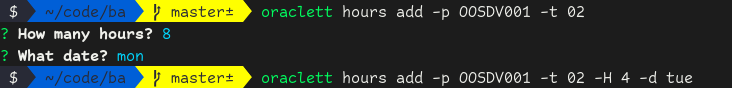
\includegraphics[scale=0.55]{hours-add.png}
  \caption{Loggen von Stunden. Beim Weglassen von Flaggen werden die Werte interaktiv erfragt.}
  \label{lst:hour-add}
  \label{fig:hours-add}
\end{figure}

Auch Notizen, dazu woran gearbeitet wurde, können unkompliziert mit
\codeinline{note add} niedergeschrieben werden.

\begin{figure}[H]
  \centering
  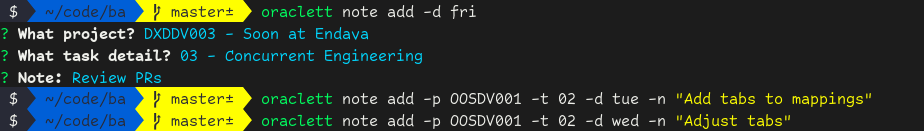
\includegraphics[scale=0.5]{note-add.png}
  \caption{Hinzufügen von Notizen. Beim Weglassen von Flaggen werden die Werte auch hier interaktiv erfragt.}
  \label{fig:note-add}
\end{figure}

Zum Abschluss der Arbeitswoche würde mit \codeinline{timecard} ein Report
erstellt, dessen Daten dann in das interne Oracle System übertragen werden.

\begin{figure}[H]
  \centering
  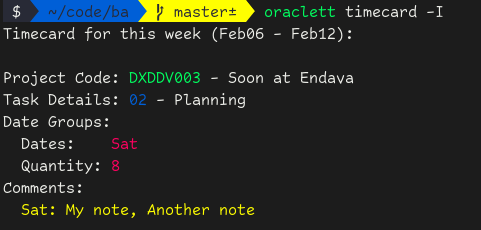
\includegraphics[scale=0.6]{timecard-ideal.png}
  \caption{Ein die ganze Woche zusammenfassender Report. Die Struktur ist darauf optimiert in die Web-Oberfläche von Oracle übertragen zu werden.}
  \label{fig:timecard}
\end{figure}

Zum Verwalten oder Ausbessern der Daten im System gibt es jetzt noch die
\codeinline{edit} und \codeinline{remove} Subkommandos. Diese stehen falls
benötigt zur Verfügung, sind aber nicht Teil des normalen Workflows.

\begin{figure}[H]
  \centering
  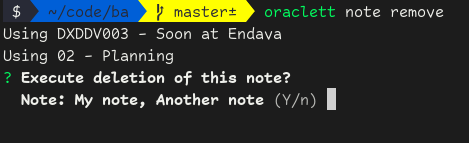
\includegraphics[scale=0.5]{note-remove.png}
  \caption{Das Löschen einer Notiz}
  \label{fig:note-remove}
\end{figure}

Die Farben für verschiedene Daten sind über alle \codeinline{list} Subkommandos
einheitlich gehalten. So sind die Referenzcode von Projekte und `Task
Details' Grün bzw. Blau\footnote{Siehe Abbildungen \ref{fig:project-add},
\ref{fig:project-list}, \ref{fig:note-add}, \ref{fig:timecard},
\ref{fig:note-list} und \ref{fig:hour-list}.}. Notizen sind in Gelb
markiert\footnote{Siehe Abbildungen \ref{fig:note-add}, \ref{fig:timecard}
und \ref{fig:note-list}.} und die Anzahl von Stunden sowie Wochentage werden
mit Magenta hervorgehoben\footnote{Siehe Abbildungen \ref{fig:hours-add},
\ref{fig:note-add}, \ref{fig:timecard}, \ref{fig:note-list} und
\ref{fig:hour-list}.}.

\begin{figure}[H]
  \centering
  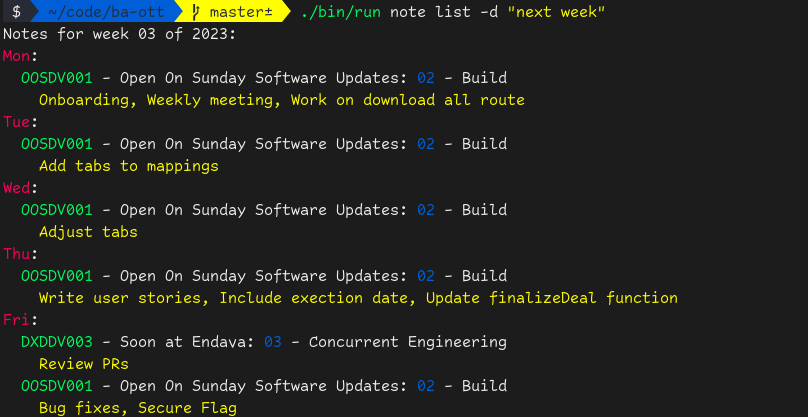
\includegraphics[scale=0.65]{note-list.png}
  \caption{Die Auflistung der Notizen einer gewählten Woche.}
  \label{fig:note-list}
\end{figure}

\begin{figure}[H]
  \centering
  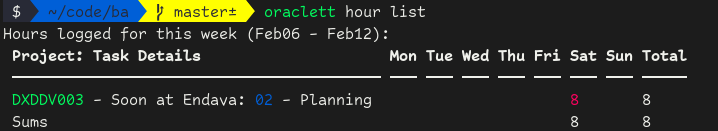
\includegraphics[scale=0.55]{hour-list.png}
  \caption{Die Auflistung aller geloggten Stunden für die aktuelle Woche.}
  \label{fig:hour-list}
\end{figure}

Die Anwendung ist über npm\footnote{Den `Node Package Manager'.} als
\href{https://www.npmjs.com/package/oraclett}{Paket verfügbar}: \codeinline{npm
install -g oraclett}. Und funktioniert auch problemlos unter Windows.

\chapter{Implementation der Methoden}
\label{sec:implementation}

Die im Kapitel \ref{sec:methods} erarbeiteten Methoden wurden in der, im
vorherigen Kapitel vorgestellten, `Time tracking` Anwendung implementiert.
Dieses Kapitel hebt hervor wie die Methoden implementiert werden können und
welche Probleme ggf. zu beachten sind.

\section{Flaggen anstatt Argumenten}
\label{sec:impl_flags_over_args}

Wie schon im Hilfsmenü von \codeinline{hour add} zu sehen war (vgl. Listing
\ref{lst:hour-add}) werden alle Werte als Flaggen erwartet.

Neben dem Wegfallen der Reihenfolge sind die Flaggen auch elementar für das
Zusammenspiel mit anderen Methoden. Wenn der Nutzer von Defaultwerten Gebrauch
machen will oder nach fehlenden Werte interaktiv gefragt werden will, kann die
spezifische Flagge einfach weg gelassen werden. Mit Argumenten wäre dies so
nicht möglich gewesen.

\section{Unterstützung aller Hilfs- und Versionsflaggen}

Bezüglich \methref{support_all_help_version} wurden alle gängigen Varianten
unterstützt.

Mit oclif war dies sogar sehr einfach (\codeinline{--help} und
\codeinline{--version} sind standardmäßig unterstützt):
\begin{code}
  \begin{javascriptcode}
..
"oclif": {
  "additionalHelpFlags": [
    "-h",
    "help"
  ],
  "additionalVersionFlags": [
    "-v",
    "-V",
    "-version"
    "version"
  ],
  ..
  \end{javascriptcode}
  \captionof{listing}{Konfiguration von Hilfs- und Versionsflaggen für oclif in der \codeinlinefn{package.json}.}
  \medskip
\end{code}

\section{Relevante Standardwerte}
\label{sec:impl_defaults}

\methref{relevant_defaults} wurde auf zwei Wegen implementiert. Einmal exakt wie
vorgesehen und einmal als Weiterführung im Sinne der Methode.

\medskip
\smallskip
\begin{code}
  \begin{shellcode}
-d, --date=<value>  [default: this week] A date to specify the week
                    (can be human-readable)
  \end{shellcode}
  \captionof{listing}{Eine mit Default versehene \codeinline{--date} Flagge.}
  \medskip
\end{code}

Der Überstehende Auszug aus dem Hilfsmenü von \codeinline{hour list}
kommuniziert das die \codeinline{--date} Flagge, sollte diese nicht übergeben
werden, den Wert \codeinline{this week} annimmt. Wird das Subkommando
\codeinline{hour list} ohne Flaggen aufgerufen, werden die Stunden der aktuellen
Woche angezeigt. Natürlich kann auch ein anderer Zeitraum angegeben werden, aber
die aktuelle Woche wird für die meisten Nutzer am relevantesten sein.

\bigskip

In manchen Fällen besteht nur eine Auswahlmöglichkeit. Diese wird dann
automatisch ausgewählt ohne den Nutzer interaktiv danach zu fragen. Natürlich
muss dieser darüber auch informiert werden. Am Beispiel von \codeinline{hour
edit} in der Abbildung \ref{fig:hours-edit-defaults} gestaltet sich das wie
folgt: Der Standardwert für das Datum ist \codeinline{today}. In diesem Falle
wurden `heute' nur Stunden für eine einzige Projekt-`Task Detail' Kombination
festgehalten und diese wird deshalb direkt ausgewählt.

\begin{figure}[H]
  \centering
  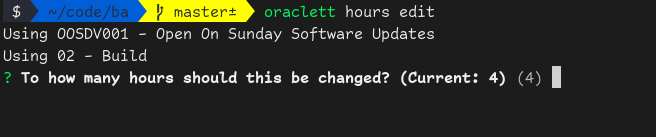
\includegraphics[scale=0.6]{hours-edit-defaults.png}
  \caption{Wenn nur eine Option zur Auswahl steht wird diese automatisch verwendet.}
  \label{fig:hours-edit-defaults}
\end{figure}

Und wenn am gewählten Tag keine Stunden (oder Notizen) festgehalten wurden,
wird in den Wochenmodus gewechselt. Dieser erlaubt, wie auch in Abb.
\ref{fig:day-week-mode} zu sehen, das Auswählen eines Wochentages für den
Stunden vorhanden sind.

\begin{figure}[H]
  \centering
  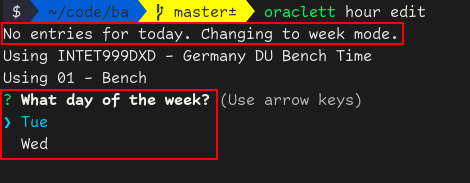
\includegraphics[scale=0.6]{day-week-mode.png}
  \caption{Wechseln vom Tagesmodus in den Wochenmodus, welcher aus Wochentagen mit vorliegenden Daten auswählen lässt.}
  \label{fig:day-week-mode}
\end{figure}

Außerdem wurden eine Auswahl an häufigen geteilten Projekten eingebettet. Der
Nutzer hat immer noch die Möglichkeit diese zu entfernen, aber wahrscheinlich
werden diese von allen Anwendern früher oder später einmal benötigt. Darunter
sind u.a. Projekt Codes zum absolvieren von Trainings, internen Events und der
Bank (keinem kommerziellen Projekt zugeordnet).

\section{Interaktives Nachfragen bei fehlendem Parameter}

Wie schon in Abbildung \ref{fig:hours-add} und \ref{fig:note-add} zu
sehen, wurde \methref{interactive_missing_param} konsequent umgesetzt.
So werden, wie auf den Abbildungen zu sehen, die fehlenden Angaben
erfragt. Wie schon angesprochen ist das so aber nur im Zusammenspiel mit
\methref{flags_over_arguments} (vgl. Kap. \ref{sec:impl_flags_over_args})
möglich.

Es wurde insbesondere vom Auswählen aus einer Liste von Werten Gebrauch gemacht
(wie in Abb. \ref{fig:hours-add} zu sehen), da es sehr intuitiv ist.

\section{Natürliche Sprache}
\label{sec:sol-natural-lang}

% TODO: write impl wit libraby (Keine Empfehlung)

Die \methref{human_language} wurde primär durch das Verarbeiten von
Datumsangaben in natürlicher Sprache implementiert. So kann anstatt starrer
Formate wie \codeinline{MM/DD/YY} einfach \codeinline{Monday} geschrieben
werden, wenn der Montag dieser Woche gemeint ist.

\begin{code}
  \begin{shellcode}
  mon, last monday, monday two weeks ago, today, yesterday, tomorrow, aug 14
  \end{shellcode}
  \captionof{listing}{Unterstützte Varianten der Datumsangabe.}
  \medskip
\end{code}

Eingaben wie \codeinline{Monday} oder \codeinline{yesterday} sind keine
absoluten Datumsangaben, sondern steht immer im Kontext dazu wann der Befehl
ausgeführt wird. Da aber der Fokus der Anwendung auf der aktuellen bzw. der
vergangenen Woche liegt besteht darin kein Problem. In der Evaluation zeigten
sich die Nutzer zufrieden damit auf diesem Wege Daten zu beschreiben. Absolute
Datumsangaben werden aber natürlich auch unterstützt. Umgesetzt wurde das
Ganze mit der Library \href{https://sugarjs.com/dates/}{sugar.js} (keine
Empfehlung\footnote{Keine Updates seit 4 Jahren. Auch sind im späteren Teil des
Bauens ein paar `Edgecase' Fehler aufgefallen.}).

\bigskip

Auch sollten Synonyme für Subkommandos ``erkannt'' werden. Angedacht war das
Einrichten von alternativen Namen bzw. Aliasen. So sollten Subkommandos
wie \codeinline{hour} auch als \codeinline{hours} erkannt werden. Oder
\codeinline{remove} als \codeinline{delete}, etc. Leider wurde dies von oclif
nur inkonsequent und verwirrend unterstützt. So können Flaggen ganz einfach mit
einem Alias versehen werden. Auch Kommandos haben diese Option, dabei würde aber
folgendes heraus kommen:

\begin{code}
  \begin{minted}[
    linenos,
    numbersep=6pt,
    frame=lines,
    framesep=2mm,
    fontsize=\footnotesize,
    highlightlines={2,5}
  ]{shell}
  COMMANDS
  hour add     Log working hours.
  hour edit    Edit the logged hours interactively.
  hour list    List all logged hours.
  hour log     Log working hours.
  hour remove  Remove logged hours interactively.
  \end{minted}
  \captionof{listing}{Auszug aus dem Hilfsmenü von \codeinlinefn{hour}. Subkommandos \codeinlinefn{add} und \codeinlinefn{log} teilen die gleiche Beschreibung.}
  \medskip
\end{code}

Kommandos die als Alias markiert sind tauchen immer in den Hilfsseiten auf.
Dadurch wird die Liste weniger übersichtlich und hilfreich. Der Nutzer weiß
nicht was der Unterschied ist. Es gibt aber von oclif aus keinen Weg diese zu
verstecken. Weshalb sich gegen diese potenziell frustrationssparenden Aliase
entschieden wurde.

\section{Fehlerkorrektur}

\begin{figure}[H]
  \centering
  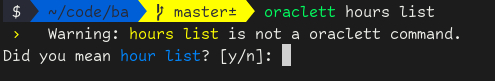
\includegraphics[scale=0.6]{did-you-mean.png}
  \caption{Beispiel der `Meintest du ..' Fehlerkorrektur.}
  \label{fig:did-you-mean}
\end{figure}

Um dem Nutzer bei Tippfehler trotzdem einen schnellen Weg zum
Ausführen des richtigen Befehls zu geben, wurde im Bezug auf
\methref{typos} eine suggestive Fehlerkorrektur eingebaut (siehe
Abb. \ref{fig:did-you-mean}.) Diese kommt mitgeliefert als
\href{https://www.npmjs.com/package/@oclif/plugin-not-found}{Plugin} für oclif.

\bigskip

Synonyme wie die im letzten Kapitel (\ref{sec:sol-natural-lang}) besprochenen
\codeinline{hour} $\leftrightarrow$ \codeinline{hours} die sich sehr ähnlich
sind können durch auch die Fehlerkorrektur verbessert werden (siehe Abb.
\ref{fig:did-you-mean}.) Weiter entfernte Synonyme wie \codeinline{remove}
$\leftrightarrow$ \codeinline{delete} funktionieren leider nicht. Da dem System
wahrscheinlich auch keine Synonymdatenbank unterliegt.

\section{Autovervollständigung}
\label{sec:impl-autocomplete}

Die \methref{autocomplete} und die damit verbundene Autovervollständigung sind
technisch gesehen implementiert, praktisch aber nicht nutzbar:

\begin{figure}[H]
  \centering
  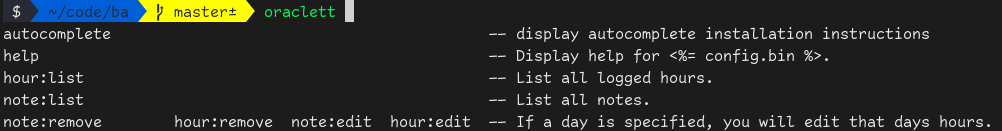
\includegraphics[scale=0.42]{apps-autocomplete.png}
  \caption{Problematisches Autovervollständigungsmenü der App}
  \label{fig:apps-autocomplete}
\end{figure}

Wie auf der Abbildung \ref{fig:apps-autocomplete} zu sehen ist existieren
einige Probleme. Am offensichtlichsten sind die Doppelpunkte (`:') zum Trennen
der Subkommandos anstatt von Leerzeichen. Das ist eine von oclif vorgegebene
Konvention und obwohl der Rest der Anwendung Leerzeichen nutzt (die auch
viel weiter verbreitet sind), sind die Doppelpunkte an dieser Stelle nicht
konfigurierbar. In der letzten Zeile wird als Beschreibung etwas von ``If a
day is specified [..]'' geschrieben. Es wurde unerklärlicherweise nicht die
Zusammenfassung verwendet sondern ein Schnipsel aus dem Hilfsmenü. Welcher
an dieser Stelle nur verwirrend für den Nutzer ist. Und zuletzt wird in der
Beschreibung der ersten Zeile der Beginn des Satzes nicht großgeschrieben und
in der zweiten Zeile der Template String nicht evaluiert. Alle dieser Dinge
sind nicht konfigurierbar. Für eine ordentliche Vervollständigung müsste diese
also selbst gebaut werden. oclif erschwert dies aber für externe Libraries wie
\href{https://github.com/f/omelette/issues/52}{omelette}. Und die Completion
Dateien selbst in Shell zu schreiben, ohne den Zugriff auf die Quellcode Dateien
welche die Struktur und Inhalte vorgeben, wäre sehr fehleranfällig.

Die geringe Qualität dieser Autovervollständigung war beim initialen Testen
des Frameworks und dem Lesen der Dokumentation noch nicht ersichtlich.
Und nach der Implementation war es zu spät zu einem anderen Framework zu
wechseln\footnote{Mögliche Alternativen wurden im Kapitel \ref{sec:oclif}
aufgeführt.}, bei welchem möglicherweise eine bessere Autocompletion möglich
gewesen wäre.

Um Verwirrung bei den Endnutzern zu vermeiden wurde die Funktionalität wieder aus
der App entfernt.

\section{Menü-basiertes Interface}
\label{sec:impl-menu}

Bei \methref{menu} wurde sich aufgrund des zeitlichen Rahmens gegen
eine Implementierung entschieden. Das Interface wäre von dem primären
Kommandozeilen-Interface gänzlich abgetrennt. Die Implementation und das
gewährleisten einer einheitlichen Nutzungserfahrung die über beide Interfaces
hinweg würde einen, im Vergleich zum Rest der App, unverhältnismäßigen Aufwand
mit sich bringen. Die Anforderungen hätten aber durchaus als Menü abgebildet
werden können.

\section{Relevante Kommandovorschläge}

\methref{command_recommendations} hat in der App keine Anwendung gefunden. Wie
auch in der Erklärung wiedergegeben spricht \textcite{dutta} diese Empfehlung in
Hinsicht auf CLI Apps mit sehr vielen (Sub-) Kommandos aus. Die implementierte
Anwendung umfasst nur eine sehr limitierte Anzahl von Subkommandos. Aufgrund
dieser bereits gegebenen Übersichtlichkeit wurde sich gegen die direkten
Vorschläge entschieden.

In den Fehlermeldungen wurde der Geiste der Methode aber angewandt. So verweist
ein fehlendes Projekt etwa auf das Hinzufügen und Auflisten von Projekten hin
(siehe nachstehende Abbildung.)

\begin{figure}[H]
  \centering
  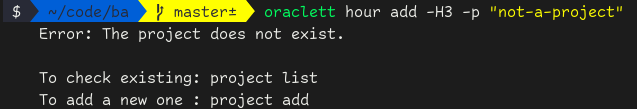
\includegraphics[scale=0.5]{recommendation-invalid-project.png}
  \caption{Vorschläge zum Hinzufügen und Auflisten von Projekten bei Angabe eines invalides Projektnamens.}
  \label{fig:recommendation-invalid-project}
\end{figure}

\chapter{Evaluation}
\label{sec:evaluation}

Im Rahmen der Studie beziehen sich GUI oder GUI App immer auf die Oracle Webapp.
Gleichermaßen steht es um CLI oder CLI App, mit welchem immer die im Rahmen der
Arbeit gebaute \codeinline{oraclett} Anwendung gemeint.

\section{Design der Studie}

Es wurde ein Usability-Test durchgeführt. Laut \cite[36]{hegner2003} werden
dabei ``[..] konkrete Nutzungssituationen durch repräsentative Endnutzer
simuliert, um die Bedienbarkeit eines Produkts oder Prototypen zu überprüfen.''
Es wurde die implementierte CLI App der existierenden GUI Webapp gegenüber
gestellt. Die Teilnehmer haben in beiden Apps Aufgabenstellungen erfüllt und
dann die Attraktivität der Applikation bewertet. Das Ziel war es zu sehen
welchen Effekt die entwickelten und implementierten Methoden auf die Nutzbarkeit
des CLI hatten. Ob die, der Kommandozeile inhärente, Nutzungsschwelle abgesenkt
werden konnte. Die existierende GUI Webapp diente dazu als Maßstab gegen welchen
es die Usability und Performance des CLI zu vergleichen galt.

\subsection{Rahmenbedingungen}

Die Teilnehmer der Studie waren alle Mitarbeiter der Firma Endava. Dies
war eine Voraussetzung um die Zugriffsrechte für die Nutzung der internen
Oracle Platform, mit welcher verglichen werden sollte, zu gewährleisten.
Die Teilnehmer waren mehr oder weniger mit dem zum Vergleich stehenden GUI
System vertraut\footnote{Von mehreren Jahren bei Endava bis zu wenigen
Wochen.}. Und hatten dieses schon für die zu testenden Tätigkeiten verwendet.
Das Verständnis der Anwendungsdomäne der Apps war also gegeben. Alle
Teilnehmer waren Software Entwickler oder Entwicklungsnah. Expertise mit der
Kommandozeile war zwischen ``wird nur benutzt wenn es nicht anders geht'' und
``wird regelmäßig verwendet''. Insgesamt wurden 6 Personen getestet. Laut
\textcite[11]{Spolsky_2001} ist ``[..] five or six users [..] all you need.''.
Durchgeführt wurde der Test via Videoanruf mit geteiltem Bildschirm. Die
Teilnehmer arbeiteten das erste Mal mit der CLI App. Um Erlernbarkeit zu testen
und trotzdem vergleichbare Performancemetriken zu erhalten wurde den Teilnehmern
eine Einführung in die Anwendung gegeben. In welcher alle Funktionalität gezeigt
und beschrieben wurde. Inklusive einem `Refresher' zum Auffinden von Hilfe
und Shell Basics wie \codeinline{CTRL+c}\footnote{Unterbricht die interaktive
Eingabe.} und Anführungszeichen um gruppieren von Text\footnote{Text mit
Leerzeichen muss in der Shell gruppiert werden: \codeinlinefn{-d "next monday"}
$\leftrightarrow$ \codeinlinefn{-d next monday}. Der zweite Aufruf führt zu
einem Fehler, weil die App denkt \codeinlinefn{monday} wäre als Argument
übergegen.}. Alles um zu gewährleisten das die Teilnehmer, ohne das Eingreifen
des Testleiters, die gegebenen Aufgaben lösen können.

\subsection{Aufgabenstellungen}
\label{aufgaben}

Es sollten die gleichen Aufgaben in beiden System erledigt werden. Um die beiden
Apps vergleichbar zu machen, wurde nur die Schnittmenge der Funktionalitäten
beim Erstellen der Aufgaben berücksichtigt. Die zu testende Funktionalität
wurde dementsprechend auf das Verwalten von Stunden und Notizen beschränkt. In
Hinsicht auf die Erlernbarkeit wurde auf Anraten von Prof. Israel eine Menge von
20 Aufgaben gewählt.

Die Studie wurde auf Englisch durchgeführt. Um die sprachlichen Feinheiten nicht
zu vertuschen, wurden die Aufgaben hier im originalen Wortlaut wiedergegeben.
Die Teilnehmer hatten zu jeder Aufgabe auch noch Informationen dazu, auf welche
Projekte-`Task-Details' Kombination die Aufgabe Bezug nimmt.

\begin{enumerate}
  \item Add 8 hours for today on the Bench.
  \item Describe that you worked on ``Self-Learning'' during that time today.
  \item Add another 8 hours for tomorrow on the Bench.
  \item Change the 8 hours for tomorrow to 6.
  \item Remove the 6 hours for tomorrow.
  \item Log 2 hours on the Bench for Friday this week.
  \item Add 6 hours on ``People Development - Certification'' for Friday this week.
  \item Describe that you did a ``Node.js Certificate'' in the hours you just logged.
  \item Change todays 8 hours on the bench to 2.
  \item And delete your note (``Self-Learning'') for today.
  \item Add 4 hours of Dev Discipline for today.
  \item Add 4 hours of Testing Discipline for today.
  \item Add 3 hours of both Testing Discipline and Dev Discipline for Monday of this week.
  \item Log 6 hours on the bench for Monday, Tuesday and Wednesday of next week.
  \item Add a note for Monday of next week that you ``Played around with Golang''.
  \item Change the just added note to ``Played around with Rust''.
  \item Change the hours for next weeks Tuesday and Wednesday to 8.
  \item Delete the hours logged for next weeks Wednesday.
  \item Show and tell Jonathan how many hours you worked in total for this week.
  \item Show and tell Jonathan how many hours you logged for the Bench next week.
\end{enumerate}

Die Häufigkeit der einzelnen Subkommandos basiert darauf wie häufig diese circa
in realer Nutzung auch auftreten würden.

Die Auflistung nach Häufigkeit:
\label{text:anzahl-aufgaben}
\begin{itemize}
  \item 8x: \codeinline{hour add}
  \item 3x: \codeinline{note add}
  \item 3x: \codeinline{hour edit}
  \item 2x: \codeinline{hour remove}
  \item 2x: \codeinline{hour list}
  \item 1x: \codeinline{note edit}
  \item 1x: \codeinline{note remove}
\end{itemize}

Um das Spielfeld etwas zu ebnen, wurde nicht immer der gleiche Wortlaut für
Verben wie `remove' verwendet. Sondern auch das synonyme `delete'. Die CLI App
verwendet aber das Verb \codeinline{remove} als Subkommando. Und dies führte
dazu das Teilnehmer u.a. versuchten \codeinline{hour delete} zu nutzen. Andere
Beispiele für diese Synonyme sind `describe' $\leftrightarrow$ `add', `change`
$\leftrightarrow$ `edit' und `log' $\leftrightarrow$ `add'. Die Sätze meinen
immer noch dasselbe, fordern die Teilnehmer bei der Verwendung des CLI aber
etwas mehr heraus.

Aufgrund der unterschiedlichen Einschränkungen der beiden User Interfaces waren
manche Aufgaben mit dem einen oder anderen theoretisch einfacher zu erledigen.
In der Auswertung wird auf diese Effekte bei spezifischen Aufgaben genauer
eingegangen.

\subsection{Zu erhebende Daten}

\subsubsection{Performance}

Um die Performance zu messen wurde festgehalten wie lange ein Benutzer benötigt
um eine gegebene Aufgabe zu erfüllen. Dazu wurden die Sitzungen aufgezeichnet
und danach mit Zeitmarken versehen. Der Zeitstempel zum Start wurde nach dem
Lesen der Aufgabe (bei erster Interaktion mit dem Interface) gesetzt und der
Zeitstempel zum Ende nach Erfüllung der Aufgabe.

\subsubsection{Attraktivität}

Um eine subjektive Bewertung des Interfaces zu erhalten wurde eine
Attraktivitätsumfrage nach \textcite{attrakdiff} durchgeführt. Es wurde nach
dem Durcharbeiten der Aufgaben für ein Interface eine Einschätzung über
dessen Attraktivität eingeholt. Wie auf Abbildung \ref{fig:survey-values}
zu sehen bewerteten die Teilnehmer dabei das Interface bezüglich mehrerer
entgegengesetzter Adjektivpaare.

\begin{figure}[H]
  \centering
  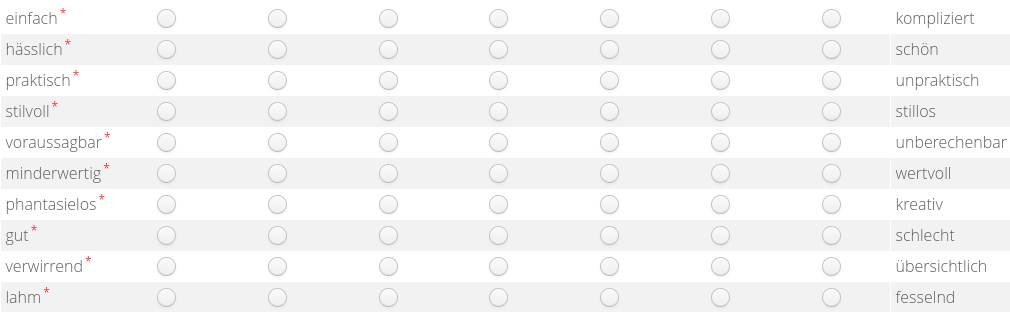
\includegraphics[scale=0.42]{survey-values.png}
  \caption{Beurteilungsbogen der kurzen AttrakDiff Umfrage.}
  \label{fig:survey-values}
\end{figure}

\subsection{Durchführung}

Nach einer generellen Einführung und Installation der App auf der Maschine des
Teilnehmers begann der Teilnehmer entweder mit der GUI Webapp oder der CLI
Applikation. 50\% der Teilnehmer begannen mit der einen, die andere Hälfte mit
der anderen. Vor der Verwendung der CLI App gab es die erläuterte Einführung.
Mit dem Hinweis darauf, dass der Versuchsleiter keine Hilfestellung leisten
würde, ging es mit der Bearbeitung der Aufgaben los. Die Checkliste der Aufgaben
waren eine nach der anderen zu bewältigen. Nach Erledigung der Aufgaben für
ein Interface folgte die Attraktivitätsumfrage, gefolgt von der Bearbeitung
derselben Aufgaben für das anderen Interface, sowie erneuter Umfrage.

\section{Hypothesen}

\newcounter{hypo}
\newcommand{\hypodef}[1]{
  \medskip
  \medskip
  \fbox{\parbox{\linewidth}{
    \refstepcounter{hypo}
    Hypothese~\thehypo: #1
    \label{hypo:\thehypo}
  }}
}
\newcommand{\hyporef}[2]{
  \medskip
  \fbox{\parbox{\linewidth}{
    \hyperref[hypo:#1]{Hypothese~#1}: #2
  }}
}

Mit den erhobenen Daten sollten folgende Hypothesen adressiert werden:

\hypodef{Das CLI hat im Durchschnitt eine ähnliche Performance wie das GUI.}
\\
Die \hyperref[sec:cli-problems]{Probleme der Kommandozeile} werden dazu führen
das Performance eingebüßt wird. Diese Probleme zu mitigieren und minimieren war
aber Zweck der Methoden. Weshalb unter Anwendung der Methoden zumindest eine
ähnliche Performance wie die einer grafischen Anwendung erwartet wird.

Nun waren die Nutzer schon mehr mit der GUI App vertraut. Gleiche Performance
bei ungleichen Startbedingungen würde sogar auf einen Performanceüberschuss
bei gleichen Startbedingungen hindeuten (i.e. wenn die Teilnehmer mit beiden
Anwendungen gleich vertraut sind.)

\hypodef{Die Performance des CLI verbessert sich im Verlaufe der Aufgaben.}
\\
Von einer erlernbaren Anwendung wäre zu erwarten das sich deren Performance
steigert wenn man den Teilnehmer genug Zeit gibt diese zu erlernen.

Zu betrachten ist die Performance ähnlicher Aufgabestellungen.

\hypodef{Das CLI wird dem GUI subjektiv vorgezogen.}
\\
Bei \textcite{Westerman_1997} wurde das CLI bei freier Wahl des Interface
deutlich weniger gewählt. Die Bevorzugung des CLI gegenüber dem GUI unter den
Teilnehmern würde also den Effekt der Methoden auf die Usability aufzeigen.

\section{Auswertung}
\label{sec:auswertung}

\subsection{Diskussion der Ergebnisse}

Über alle Diagramme hinweg ist Blau auf die Farbe der CLI App bzw. Orange die
der GUI App.

\begin{figure}[H]
  \centering
  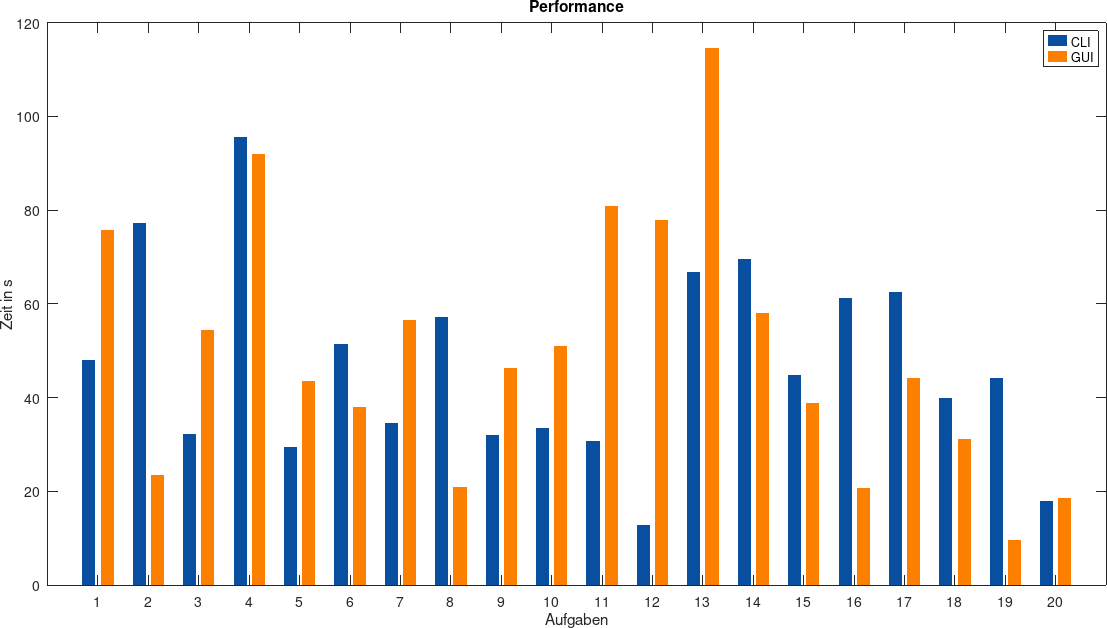
\includegraphics[scale=0.36]{performance.png}
  \caption{Performance beider Interfaces bei der Erfüllung gleicher Aufgaben.}
  \label{fig:performance}
\end{figure}

Die Performance der verschiedenen Aufgaben schwanken stark zwischen den Aufgaben
bei gleichem Interface (vgl. Abbildung \ref{fig:performance}.) Das begründet
sich darin das die Aufgaben innerhalb der gleichen Anwendung unterschiedlich
schwer zu lösen waren.

\medskip

\begin{figure}[H]
  \centering
  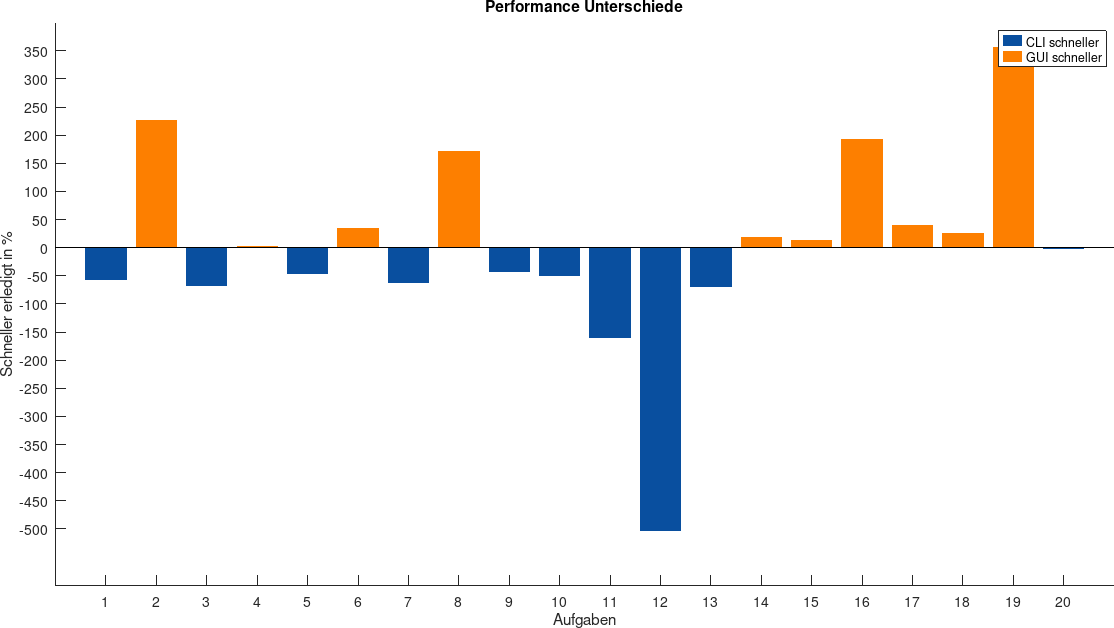
\includegraphics[scale=0.36]{performance-diff.png}
  \caption{Performance Unterschiede zwischen den Anwendungen.}
  \label{fig:performance-diff}
\end{figure}

Auch die Performance Differenz zwischen den beiden Anwendungen schwankt
(vgl. Abbildung \ref{fig:performance-diff}.) Was seine Gründe darin hat das
die Aufgabe durch ein Interface effizienter erledigt werden konnte. Für das
Kommandozeilen Interface spielt noch mit hinein das bei neuen Aufgabenstellungen
(solche die ein neues Subkommando oder eine neue Flagge erfordern) dem Nutzer
nicht klar ist, wie vorzugehen ist. Und dort Zeit für das Lesen von Hilfsmenüs
aufgewendet werden muss. Was aber in der Natur des CLI liegt.

Das Nachschauen im Hilfsmenü ist einer der Faktoren weshalb das CLI
beispielsweise bei der zweiten Aufgabe die dreifache Zeit zur Erfüllung
brauchte. Es stellte die erste Verwendung von \codeinline{note add} dar. Hinzu
kommt, dass das Hinzufügen von Notizen im GUI relativ unkompliziert ist.
Verglichen mit der zweiten Verwendung in Aufgabe 8 bleibt die Performance des
GUI fast gleich während das CLI zulegt (etwa $30\%$\footnote{Im Vergleich zur
GUI Performance. Von $225\%$ schneller Erledigung zu $160\%$.} schneller als
zuvor.)

Ebenso sind auch die Differenzen der Aufgaben 19 und 20 zu erklären. Das
erste bzw. zweite Mal das \codeinline{hour list} verwendet wurde. Von $355\%$
schnellerer GUI Performance zum gleichauf sein in der nächsten Aufgabe.

Die extremste Differenz ist bei Aufgabe 12 entstanden. Bei den Aufgaben 11 und
12 werden vier Stunden für dasselbe Projekt auf verschieden `Task Details'
festgehalten. Im GUI bleibt der Aufwand fast gleich während er sich für das
CLI halbiert und im Vergleich zum GUI zu $500\%$ schneller Performance führt.
Bei optimaler Verwendendung kann im Kommandozeilen-Interface der gleiche
Befehl für beide Aufgaben wiederverwendet werden \footnote{Der optimale Befehl
ist: \codeinlinefn{hour add -H 4 -d today -p INTDS999DXD} und es wird nur
das richtige Task Detail aus der Liste ausgewählt. Alternativ wäre auch das
Spezifizieren von \codeinlinefn{-t 08} bzw. \codeinlinefn{-t 12} ähnlich
schnell.}.

Aufgabe 16 stellt den letzten der Extremfälle dar und ist das einzige Auftritt
des \codeinline{edit} Subkommandos\footnote{Wie in Kap. \ref{text:noun-verb}
erläutert hat \codeinlinefn{orcalett} eine `noun verb' Struktur. Sowohl
die Substantive \codeinlinefn{project}, \codeinlinefn{hour} und
\codeinlinefn{note} bieten jeweils ein \codeinlinefn{edit} Subkommando an.}.

\begin{figure}[H]
  \centering
  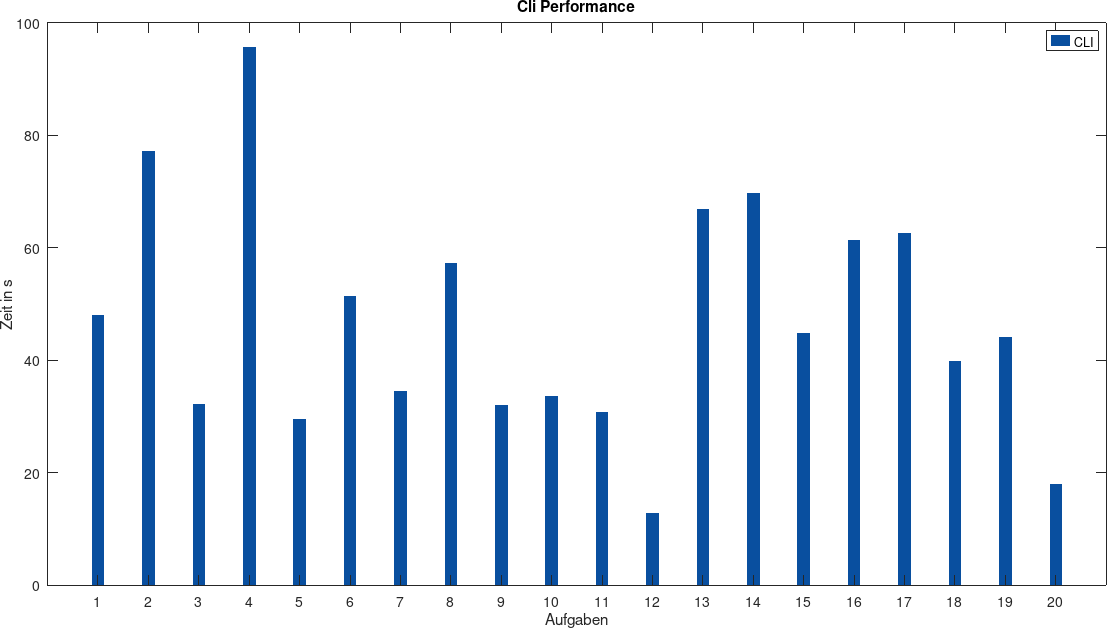
\includegraphics[scale=0.36]{performance-cli.png}
  \caption{Isolierte Performance der CLI App.}
  \label{fig:performance-cli}
\end{figure}

\begin{figure}[H]
  \centering
  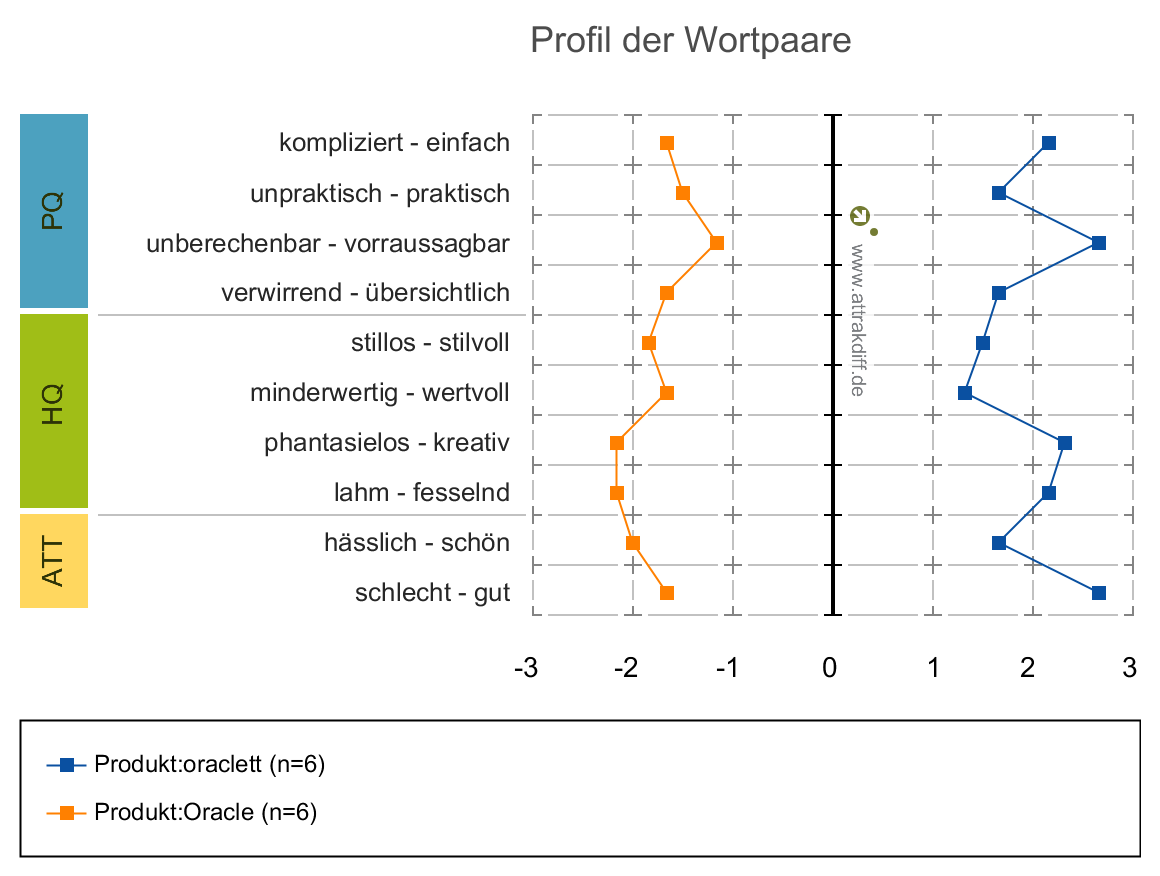
\includegraphics[scale=0.35]{attrak-wortpaare.png}
  \caption{Ergebnisse der Attraktivitätsumfrage darüber wo die Anwendungen für die einzelnen Adjektivepaare landeten.}
  \label{fig:attrak-wortpaare}
\end{figure}

\begin{figure}[H]
  \centering
  \begin{minipage}[b]{0.4\textwidth}
    \centering
    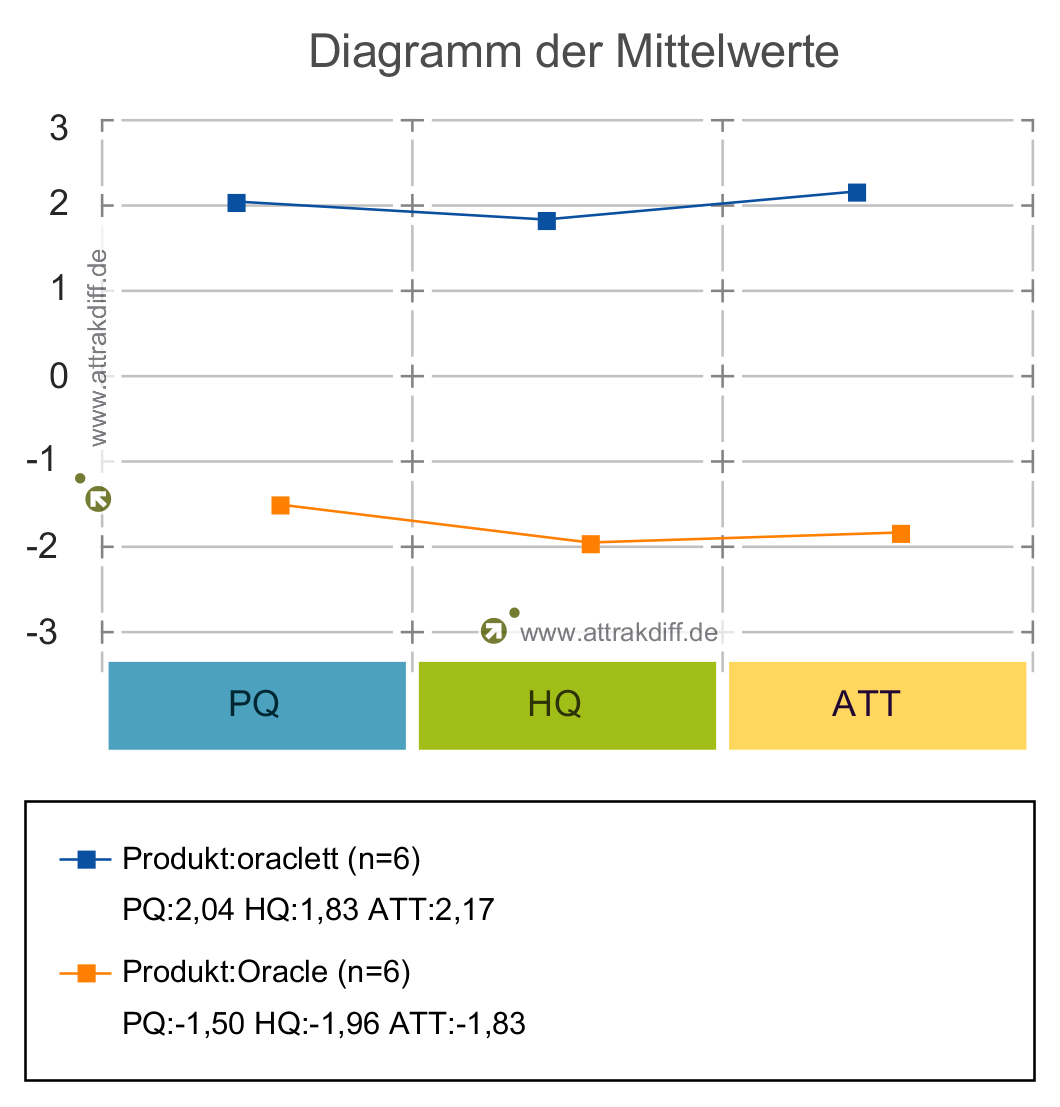
\includegraphics[scale=0.28]{attrak-mittelwerte.png}
    \caption{Mittelwerte über die von \textcite{attrakdiff} definierten Kategorien.}
    \label{fig:attrak-mittelwerte}
  \end{minipage}
  \hfill
  \begin{minipage}[b]{0.4\textwidth}
    \centering
    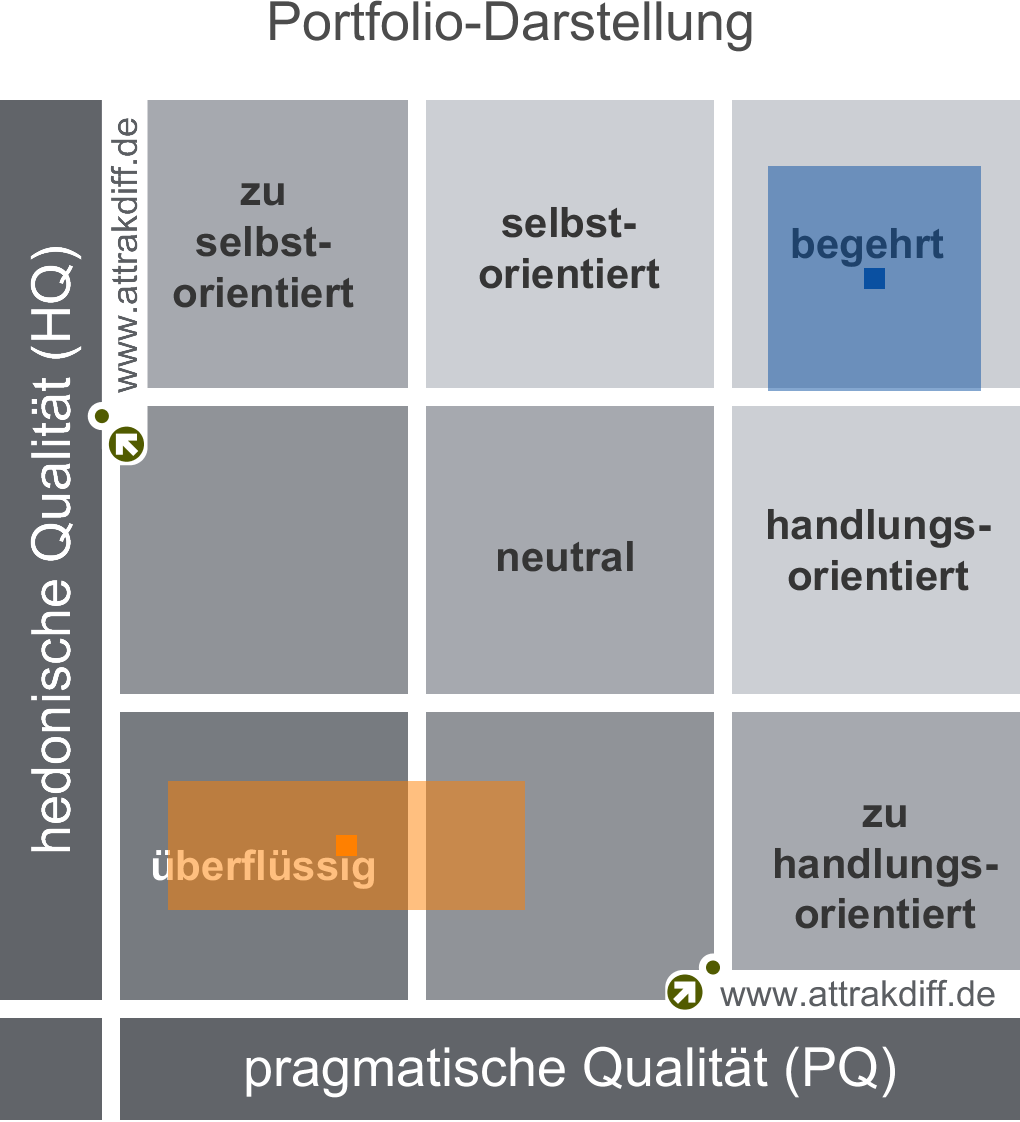
\includegraphics[scale=0.26]{attrak-portfolio.png}
    \caption{Einordnung der Ergebnisse in die Matrix nach hedonischer und pragmatischer Qualität.}
    \label{fig:attrak-portfolio}
  \end{minipage}
\end{figure}

Wie in Abbildung \ref{fig:attrak-mittelwerte} zu sehen ist, sind die Anwendungen
in allen Kategorien über $3.5$ Punkte auseinander. Auf einer Skala die nur $7$
Punkte breit ist, ist das eine Menge.

In Abbildung \ref{fig:attrak-portfolio} ``spiegelt das Konfidenz-Rechteck
[..] wieder, wie ``einig'' sich die Nutzer bei der Beurteilung
des Produkts sind. Je größer das Konfidenz-Rechteck ist, desto
unterschiedlicher wird das Produkt bewertet.'' - \textcite{attrakdiff} via
\href{https://esurvey.uid.com/}{esurvey.uid.com}.

\subsection{Auswertung der Hypothesen}

\subsubsection{Hypothese 1}
\hyporef{1}{Das CLI hat im Durchschnitt eine ähnliche Performance wie das GUI.}
\\
Der Performance Durchschnitt über alle Aufgaben aufsummiert liegt bei
$-2.76 s$, das CLI ist also um \~3 Sekunden schneller. Wie in Abbildung
\ref{fig:performance-diff} zu sehen ähnelt sich die Performance beider
Anwendungen. Keine der beiden ist konsistent schneller als die andere. Es wurden
nur bei sechs Aufgaben mehr als $100\%$ Performance Differenz festgestellt,
also das ein Interface mehr als doppelt so schnell als das andere. Auf diese
Extremfälle wurde auch bereits einleitend eingegangen.

\subsubsection{Hypothese 2}
\hyporef{2}{Die Performance des CLI verbessert sich im Verlaufe der Aufgaben.}
\\
Bei Betrachtung der Performance des CLI (Abb. \ref{fig:performance-cli})
hinsichtlich der Erlernbarkeit sind die Aufgabenstellungen zu beachten. So
werden die Aufgaben mit der Zeit schwieriger: Es werden Projekte mit mehr als
einem Task Detail verwendet (ab 7.), das Datum wandert zu anderen Wochentagen
(ab 6.) und in die nächste Woche (ab 14.). Es werden zuvor einzelne Aufgaben
gebündelt (ab 13.), etwa das hinzufügen mehrerer Stunden an verschieden
Tagen als Teil einer Aufgabe. Auch werden kontinuierlich neue Subkommando
Kombinationen gefordert\footnote{Siehe die Auflistung der Anzahl von Aufgaben
pro Subkommando in Kapitel \ref{text:anzahl-aufgaben}.}.

Trotz all dieser erschwerenden Faktoren ist ein fallender Trend zu erkennen.

\subsubsection{Hypothese 3}
\hyporef{3}{Das CLI wird dem GUI subjektiv vorgezogen.}
\\
Der subjektive Vergleich ist ziemlich eindeutig. Die Abbildung
\ref{fig:attrak-portfolio} beschreibt die CLI App als begehrt und Oracle als
überflüssig. Auch auf Abbildung \ref{fig:attrak-wortpaare} liegt das CLI in
allen Punkten signifikant vorne.

\subsection{Beobachtungen aus der Evaluation}

In der Nutzung beider Interfaces traten bei manchen Teilnehmern Momente auf in
denen sie nicht wussten wie vorzugehen war. In der CLI App sind die Teilnehmer
als Reaktion darauf zur Hilfsseite zurückgekehrt und haben versucht sich
neu zu orientieren und den Fehler in ihrem letzten Befehl zu finden. Dabei
wurde sich nicht an den Versuchsleiter gewendet. Den Teilnehmern war bewusst,
dass sie dieses Problem allein lösen können. Bei Aussetzern von Oracle (aus
unerfindlichen Gründen) herrschte immer Verwirrung. Das Interface teilte nichts
mit und tat einfach seinen Dienst nicht. An dieser Stelle wurde immer die Hilfe
des Versuchsleiters gesucht.

\chapter{Zusammenfassung}
\label{sec:zusammenfassung}

Nach Analyse der grundlegenden Probleme der Kommandozeile, wurden neun Methoden
zur Verbesserung der Usability für Kommandozeile-Interfaces erarbeitet. Diese
wurden in einer CLI App implementiert und mit einer grafischen Anwendung mit
gleichem Funktionsumfang verglichen. Die Teilnehmer bevorzugten das CLI über das
GUI, bei gleichauf liegender Performance.

\section{Schlussfolgerungen}

Es wurde gezeigt, dass in der Kommandozeile, unter Anwendung der erarbeiteten
Methoden, Usability erreicht werden kann die es mit grafischen Anwendungen
aufnimmt.

\section{Limitationen}

Es war im Rahmen der Arbeit nicht möglich den Effekt einzelner Methoden isoliert
festzustellen. Es konnte also nur eine Aussage über alle implementieren Methoden
zusammen getroffen werden.

\section{Ausblick}
\subsection{Entwicklung und Strukturierung von Methoden}

Die Methoden könnten in stärker strukturierter Form und außerhalb des Kontextes
dieser Arbeit für sich stehend formuliert werden. Zusammen mit einer englischen
Übersetzung wären sie dadurch dann leichter referenzier- und implementierbar.
Auch könnten noch weitere Methoden entwickelt werden.

\subsection{Vergleich mit CLI App}

Anstatt des Vergleiches mit einer GUI App, würde der Vergleich mit einer
baugleichen CLI App, welche die Methoden nicht implementiert, eine stärkere
Aussagekraft bezüglich des Effektes der Methoden haben. Auch wäre es damit
möglich nur eine Methode auf einmal zu testen. Mit identischen Apps A und B,
aber B hat zusätzlich die zu untersuchende Methode implementiert.

\subsection{Verbesserung der Implementation}

In der Evaluation wurden noch einige Schwächen der Implementation entdeckt,
welche noch auszubessern sind. Auch die Versäumnissen etwa wie bei der
Autovervollständigung (vgl. Kap. \ref{sec:impl-autocomplete}), dem Menü
Interface (vgl. Kap. \ref{sec:impl-menu}) oder die fehlenden Synonyme (vgl. Kap.
\ref{sec:sol-natural-lang}) bieten noch Verbesserungsbedarf.

Eine Anbindung an Oracle selbst war im Rahmen dieser Arbeit nicht vorgesehen,
weil der Fokus auf den Methoden lag. Als zukünftige Verbesserung der App wäre
dies aufgrund der Zeitersparnis aber sinnvoll.

\subsection{Bearbeiten der Problemstellung in anderer Herangehensweise}

Die zu Beginn gestellte, offene Problemstellung war: Wie Entwicklern oder der
Allgemeintheit das CLI näher gebracht werden kann. Neben dem Verbessern der
Nutzbarkeit von CLI Applikationen, sind noch andere Herangehensweisen möglich.
Etwa das Terminal-Ökosystem zugänglicher und verständlicher zu machen. Oder
die Zugänglichkeit der Werkzeuge für nicht technisch-fokussierte Personen
verbessern. Vieles ist möglich.

\printbibliography[
heading=bibintoc,
title={Quellenverzeichnis}
]

\newpage
\chapter{Glossar}

\pagenumbering{roman}
\begin{appendix}
\chapter{Appendix}

% \section{Quell-Code}

\newpage
\thispagestyle{empty}
\noindent

\section*{Eidesstattliche Versicherung}
Hiermit versichere ich an Eides statt durch meine Unterschrift, dass ich die vorstehende Arbeit selbstst\"andig und ohne fremde Hilfe angefertigt und alle Stellen, die ich w\"ortlich oder ann\"ahernd w\"ortlich aus Ver\"offentlichungen entnommen habe, als solche kenntlich gemacht habe, mich auch keiner anderen als der angegebenen Literatur oder sonstiger Hilfsmittel bedient habe. Die Arbeit hat in dieser oder \"ahnlicher Form noch keiner anderen Pr\"ufungsbeh\"orde vorgelegen.\\
\linebreak[4]
\linebreak[4]
\linebreak[4]
\linebreak[4]
-------------------------------------------------------\linebreak[4]
Datum, Ort, Unterschrift

\end{appendix}
\end{document}
